% ************************************************************************** %
% Copyright (C)  2016  Philipp Hacker.																			 %
% Permission is granted to copy, distribute and/or modify this document			 %
% under the terms of the GNU Free Documentation License, Version 1.3				 %
% or any later version published by the Free Software Foundation;						 %
% with no Invariant Sections, no Front-Cover Texts, and no Back-Cover Texts. %
% The lincense itself can be found at <https://www.gnu.org/licenses>.        % 
% ************************************************************************** %

%LICENSE:
%CC BY-NC-SA 3.0 (http://creativecommons.org/licenses/by-nc-sa/3.0/)

% Masters Thesis 
% LaTeX Template
% Version 2.3 (25/3/16)

% This template has been downloaded from:
% http://www.LaTeXTemplates.com

% Version 2.x major modifications by:
% Vel (vel@latextemplates.com)

% This template is based on a template by:
% Steve Gunn (http://users.ecs.soton.ac.uk/srg/
%						  softwaretools/document/templates/)
% Sunil Patel (http://www.sunilpatel.co.uk/thesis-template/)

% ************************************************************************** %
% ************************************************************************** %

% START OF TEX
\documentclass[
	10pt,
	twoside,
	chapterinoneline,
	onehalfspacing, % alternatives: onehalfspacing or doublespacing
	nolistspacing, % If the document is onehalfspacing or doublespacing,
								 % uncomment this to set spacing in lists to single
	%liststotoc, % Uncomment to add the list of figures/tables/etc to toc
	%toctotoc, % Uncomment to add the main table of contents to the toc
	parskip, % Uncomment to add space between paragraphs
	headsepline, % Uncomment to get a line under the header
	english,
]{MastersDoctoralThesis} % The class file specifying the document structure

% ************************************************************************** %
% CORE USEPACKAGE HERE
\usepackage{lmodern}
\usepackage[utf8]{inputenc} % Required for inputting international characters
\usepackage[T1]{fontenc} % Output font encoding for international characters
\usepackage[autostyle=true]{csquotes}
% Required to generate language-dependent quotes in the bibliography
%\usepackage[backend=bibtex,style=authoryear,natbib=true]{biblatex}
\usepackage[backend=bibtex,natbib=true]{biblatex}
% Use the bibtex backend with the authoryear citation style
\addbibresource{bibcontents/preamble.bib} % The filename of the bibliography
\addbibresource{bibcontents/master.bib} % The filename of the bibliography
% ************************************************************************** %

% ************************************************************************** %
% MARGIN
\geometry{%
	% showframe, % show how the type block is set on the page
	paper=a4paper, % Change to letterpaper for US letter
	inner=2cm, % Inner margin
	outer=3.0cm, % Outer margin
	bindingoffset=1.5cm, % Binding offset
	top=1.5cm, % Top margin
	bottom=1.5cm } % Bottom margin
% ************************************************************************** %

% ************************************************************************** %
% THESIS INFORMATION
\date{\today} 
\thesistitle{Kinetic\ effects\ in\ RF\ discharges}
% Your thesis title, this is used in the title and abstract
\supervisor{Prof.\ Dr.\ Ralf\ Schneider}
% Your supervisor's name, this is used in the title page
\examiner{Prof.\ Dr.\ Jürgen\ Meichsner}
% Your examiner's name, this is not currently used anywhere in the template
\degree{Master\ of\ Science\ -\ Physics}
% Your degree name, this is used in the title page and abstract
\author{Philipp\ Hacker}
% Your name, this is used in the title page and abstract
\addresses{Karl-Liebknecht-Ring\ 13,\ 17491\ Greifswald}
% Your address, this is not currently used anywhere in the template
\subject{Physics}
% Your subject area, this is not currently used anywhere in the template
\keywords{plasma,\ discharge,\ kinetic,\ effect,\ physics,\ master}
\university{\href{https://www.uni-greifswald.de/en/}%
					 {Ernst-Moritz-Arndt\ University\ of\ Greifswald}}
% Your university's name and URL, this is used in the title page and abstract
\department{\href{https://physik.uni-greifswald.de/en/}%
					 {Institute\ of\ Physics}}
% Your department's name and URL, this is used in the title page and abstract
\group{\href{https://physik.uni-greifswald.de/ag-schneider/}%
			{Computational\ Sciences}}
% Your research group's name and URL, this is used in the title page
\faculty{\href{https://mnf.uni-greifswald.de/en/faculty/}%
				{Faculty\ of\ Mathematics\ and\ Natural\ Sciences}}
% Your faculty's name and URL, this is used in the title page and abstract
% ************************************************************************** %

\hypersetup{pdftitle=\ttitle} % Set the PDF's title to your title
\hypersetup{pdfauthor=\authorname} % Set the PDF's author to your name
\hypersetup{pdfkeywords=\keywordnames} % Set the PDF's keywords to your keywords

% ************************************************************************** %
% PACKAGES
\usepackage{physics}
\usepackage{mathtools}
\usepackage{amssymb}
\usepackage{upgreek}
\usepackage{esint}
\usepackage{ziffer}
\usepackage{csquotes}
\usepackage{sectsty}
\usepackage{nomencl}

%% FIGURE PACKAGES
\usepackage{float}
\usepackage{graphicx}
\usepackage{subcaption}
\usepackage{wrapfig}
\usepackage{epsfig}

%\usepackage{amsmath}
% cant use svg so easily with subcaption
% \expandafter\def\csname ver@subfig.sty\endcsname{}
% \usepackage{svg}
% ************************************************************************** %

% \usepackage{titlesec}
% \titleformat{\chapter}[display]
% 	{\normalfont\huge\bfseries}{}{0pt}{\Huge}
% 	\titlespacing*{\chapter} {0pt}{20pt}{40pt}

\newcommand{\diff}{\textnormal{d}}
\newcommand{\tenpo}[1]{10^{#1}}
\newcommand{\greek}[1]{\greektext#1\latintext}
\newcommand{\ix}[1]{_\text{#1}}
\newcommand{\imag}{\mathbf{i}}
\newcommand{\tilt}[1]{\textit{#1}}
\newcommand{\divergenz}[1]{\textit{div}\left(#1\right)}
\newcommand{\euler}{\mathnormal{e}}
\newcommand{\fett}[1]{\textbf{#1}}
\newcommand{\inexample}{\text{e.g.}}
\newcommand{\kett}{\rangle}

\renewcommand{\bra}{\langle}
\renewcommand{\grad}[1]{\textit{grad}\left(#1\right)}

% Used for signature line at 
% declaration of authorship
\newcommand{\sign}[1]{%
  \begin{tabular}[t]{@{}c@{}}
  \makebox[1.5in]{\dotfill}\\
  \strut\emph{#1}\strut%
  \end{tabular}%
}

\setlength{\parindent}{0pt}
\setlength{\nomlabelwidth}{.20\hsize}
\setcounter{chapter}{0}

\setcounter{secnumdepth}{3}
%\setsecnumdepth{subsubsection}

% DOCUMENT START
\begin{document}
%
% ************************************************ %
% RENEWCOMMANDS																		 % 
\renewcommand{\equationautorefname}{equation}			 %
\renewcommand{\figureautorefname}{figure}				   %
\renewcommand{\tableautorefname}{table} 					 %
\renewcommand{\sectionautorefname}{section}				 %
\renewcommand{\subsectionautorefname}{section}		 %
\renewcommand{\subsubsectionautorefname}{section}	 %
\renewcommand{\figurename}{\bfseries Figure}			 %
\renewcommand{\tablename}{\bfseries Table}				 %
\renewcommand{\nomlabel}[1]{#1 \dotfill}					 %
\setlength{\abovedisplayskip}{9pt}                 %
\setlength{\belowdisplayskip}{9pt}                 %
\setlength{\abovedisplayshortskip}{9pt}            %   
\setlength{\belowdisplayshortskip}{9pt}            %
% ************************************************ %
%	
	\frontmatter
  % Use roman page numbering style (i, ii, iii, iv...)
	% for the pre-content pages
	\pagestyle{plain}
  % Default to the plain heading style until the thesis style
	% is called for the body content
%
% TITLEPAGE
\begin{titlepage}
	\begin{center}
		{\scshape\LARGE \univname\par}\vspace{1.5cm} % University name
		% TODO: THESIS TYPE
		\textsc{\Large Master Thesis}\\[0.5cm]
		\HRule\\[0.4cm] % Horizontal line
		{\huge \bfseries \ttitle\par}\vspace{0.4cm} % Thesis title
		\HRule\\[1.5cm] % Horizontal line
		\begin{minipage}[htbp]{0.4\textwidth}
			\begin{flushleft}\large
				\emph{Author:}\\
				\authorname% TODO: AUTHOR NAME
			\end{flushleft}
		\end{minipage}
		\hfill
		\begin{minipage}[htbp]{0.4\textwidth}
			\begin{flushright}\large
				\emph{Supervisor:}\\
				\supname% TODO: SUPERVISOR
			\end{flushright}
		\end{minipage}\\[0.5cm]
		% TODO: UNIVERSITY TEXT
		\large \textit{A thesis submitted in fulfillment of
									 the requirements\\ for the degree of
									 \degreename}\\[0.3cm]
		\textit{in the research group of}\\[0.4cm]
		% TODO: RESEARCH GROUP/DEPARTMENT
		\groupname,\\\deptname\\[1cm]
%
		% University/department logo - uncomment to place it
		% use for pdf files
		% 
\includegraphics[width=0.50\textwidth]{figures/logos/logo_color.pdf}\\[1.0cm]
		% 
\includegraphics[width=0.55\textwidth]{figures/logos/logo.pdf}\\[1.0cm]
%
		% use for eps files
		\hspace*{0.75cm}
		
\epsfig{width=0.45\textwidth,file=figures/logos/logo.eps}\\[1.0cm]
%
		{\large \today}
		\vfill
	\end{center}
\end{titlepage}
%
% ************************************************************************** %
% DECLARATION OF AUTHORSHIP
	%
	\chapter*{Declaration of Authorship}
%
		I hereby certify that this thesis has been composed by me and is based on 
		my own work, unless stated otherwise.	No other person’s work has been used
		without due acknowledgement in this thesis.
		All references and verbatim extracts have been quoted, and iall sources of
		information, including graphs and data sets, have been specifically
		acknowledged.\\[2.0cm]
%
		\begin{flushright}
			\sign{Signature of author}\\
			Greifswald; \today
		\end{flushright}
%
% ************************************************************************** %
%
% ************************************************************************** %
%  TOCTOCTOC FOR EVERYTHING
	\tableofcontents % Prints the main table of contents
	% \listoffigures % Prints the list of figures
	% \listoftables % Prints the list of tables
% ************************************************************************** %
%
% ************************************************************************** %
% PREFIX
	% ************************************************************************** %
% INSERT ABBREVIATIONS
	\begin{abbreviations}{ll}
		\toprule
		\bfseries abbreviation & \bfseries full expression \\%
		\toprule \midrule \endhead%
		e.g.                      & exempli gratia; \emph{for example} \\ \\%
		etc.                      & et cetera; \emph{and so on} \\ \\%
        ac                        & alternating current \\ \\%
        dc                        & direct current \\ \\%
		rf, RF                    & radio frequency \\ \\%
        ccrf                      & capacitively coupled radio frequency \\ \\%
        EDF                       & energy distribution function \\ \\%
		EDV                       & \emph{german: Energieverteilungsfunktion}, energy distribution function \\ \\%
        EEDF                      & electron energy distribution function \\ \\%
        IEDF                      & ion energy distribution function \\ \\%
		p., pp.					  & page, plural pages \\ \\%
		ff.						  & folio; \emph{on the (next) page}, ablative of folium (\emph{page}) \\ \\%
		SIE, SEE			  	  & secondary ion/electron emission \\ \\%
		HWA						  & hard wall approximation \\ \\%
		MS						  & mass spectrometer \\ \\%
		PROES					  & phase resolved emission spectroscopy \\ \\%
		MWI						  & microwave interferometer \\ \\%
		AN						  & antenna \\ \\%
		FC						  & flow controller \\ \\%
		PIC						  & particle-in-cell \\ \\%
		MCC						  & Monte-Carlo-Colissions \\ \\%
		
		\midrule \bottomrule
    \caption{%
      List of abbreviations and their corresponding phrases. If specified, the translation %
      or an equivalent expression is written.}\label{tabe:abbreviations}
	\end{abbreviations}
% ************************************************************************** %

% ************************************************************************** %
% CONSTANTS AND SYMBOLS LIST
	\begin{constants}{lcccl}
		\toprule
		\bfseries Quantity & \bfseries Unit &
		\bfseries Symbol & \bfseries Dimension & \bfseries Value \\%
		\toprule \midrule \endhead%
	  Speed of Light           & $\unit{m/s}$ & $c\ix{0}$ & $\unit{L^{1}T^{-1}}$ & %
	                             $\SI{2,997}\cdot\tenpo{8}$ \\ \\%
      thermal velocity         & $\unit{m/s}$ & $v\ix{th,j}$ & $\unit{L^{1}T^{-1}}$ & \\ \\%
      drift velocity           & $\unit{m/s}$ & $v\ix{D,j}$, $u\ix{j}$ & $\unit{L^{1}T^{-1}}$ & \\ \\%
      Boltzmann constant       & $\unit{eV/K}$ & $k\ix{B}$ & $\unit{M^{1}L^{2}T^{-2}K^{-1}}$ & %
    							 $\SI{8,617}\cdot\tenpo{-23}$ \\ \\%
      mobility                 & $\unit{cm^{2}/Vs}$ & $\mu\ix{j}$ & $\unit{I^{1}T^{2}M^{-1}}$ & \\ \\%
	  planck constant          & $\unit{eVs}$ & $\hbar$ & $\unit{G^{-1/2}c^{6/2}\varepsilon\ix{0}^{1/2}}$%
							 									   & $\unit[\SI{4.1345}\cdot\tenpo{-15}]{eVs}$ \\ 
															 & & & & $\unit[\SI{6,646}\cdot\tenpo{-34}]{Js}$ \\ \\%
	  kinetic temperature      & $\unit{eV}$ & $T\ix{j}$ & $\unit{M^{1}L^{2}T^{-2}}$%
				 			   & $\unit[1]{eV}=\unit[\SI{1.902}\cdot\tenpo{-19}]{K}$ \\ \\%
 	  elementary charge        & $\unit{C}$ & $e$ & $\unit{I^{1}T^{1}}$ & $\SI{1.902}\cdot\tenpo{-19}$ \\ \\%
      electric charge          & $\unit{C}$ & $Q$, $q$ & $\unit{I^{1}T^{1}}$ & \\ \\%
	  particle mass            & $\unit{kg}$ & $m\ix{j}$ & $\unit{M^{1}}$ & %
 																				  electron: $\SI{9.109}\cdot\tenpo{-31}$ \\
															 & & & & \hspace*{.62cm}   ion: $\SI{5.310}\cdot\tenpo{-26}$ \\
															 & & & & \hspace*{.27cm} anion: $\SI{5.143}\cdot\tenpo{-26}$ \\ \\%
	  reduced mass             & $\unit{kg}$ & $\mu\ix{j,k}$ & $\unit{M^{1}}$ & \\ \\%
      distance,location        & $\unit{cm}$ & $r$, $\vec{r}$ & $\unit{L^{1}}$ & \\ \\%
	  Debye length             & $\unit{cm}$ & $\lambda\ix{D,j}$ & $\unit{L^{1}}$ & \\ \\%
	  particle distance        & $\unit{cm}$ & $\overline{b}$ & $\unit{L^{1}}$ & \\ \\%
	  mean free path           & $\unit{cm}$ & $s\ix{mfp,j}$ & $\unit{L^{1}}$ & \\ \\%
      particle density         & $\unit{cm^{-3}}$ & $n\ix{j}$ & $\unit{L^{-3}}$ & \\ \\%
      Vacuum permittivity      & $\unit{F/m}$ & $\varepsilon\ix{0}$%
							   & $\unit{M^{-1}L^{-3}T^{-4}A^{2}}$ & $\SI{8.854}\cdot\tenpo{-12}$ \\ \\%
	  electrostatic potential  & $\unit{V}$ & $\Phi$, $U$ & $\unit{M^{1}L^{2}I^{-1}T^{-3}}$ & \\ \\%
      electric current         & $\unit{As}$ & $I$, $J$ & $\unit{I^{1}}$ & \\ \\%
      electric current density & $\unit{As/cm^{2}}$ & $j\ix{j}$ & $\unit{I^{1}L^{-2}}$ & \\ \\%
      electric charge density  & $\unit{C/cm^{3}}$ & $\rho$ & $\unit{I^{1}T^{1}L^{-3}}$ & \\ \\%
    \midrule\bottomrule% pagebreak
      electric resistance      & $\unit{\Omega}$ & $R$ & $\unit{M^{1}L^{2}T^{-3}I^{-2}}$ & \\ \\%
      electric capacity        & $\unit{F}$ & $C$ & $\unit{M^{-1}L^{-2}T^{4}I^{2}}$ & \\ \\%
      time                     & $\unit{s}$ & $t$ & $\unit{T^{1}}$ & \\ \\%
      plasma frequency         & $\unit{Hz}$ & $\omega\ix{p,j}$ & $\unit{T^{-1}}$ & \\ \\%
      collisional frequency    & $\unit{Hz}$ & $\nu\ix{j}$ & $\unit{T^{-1}}$ & \\ \\%
%
		\midrule\bottomrule
    \caption{%
      Physical properties in their commonly --- or for this purpose most convenient %
      --- units and corresponding SI units. If not specified, the values of each quantity %
      refer to the afore-mentioned units.}\label{tabe:physicalconstants}
	\end{constants}
% ************************************************************************** %


% ************************************************************************** %
	\mainmatter% 
	\pagestyle{thesis}
% ************************************************************************** %
% INSERT ABSTRACT
% 
	%
	\chapter*{Motivation}\addchaptertocentry{Motivation}
%
        \begin{figure}[!b]
            \centering
            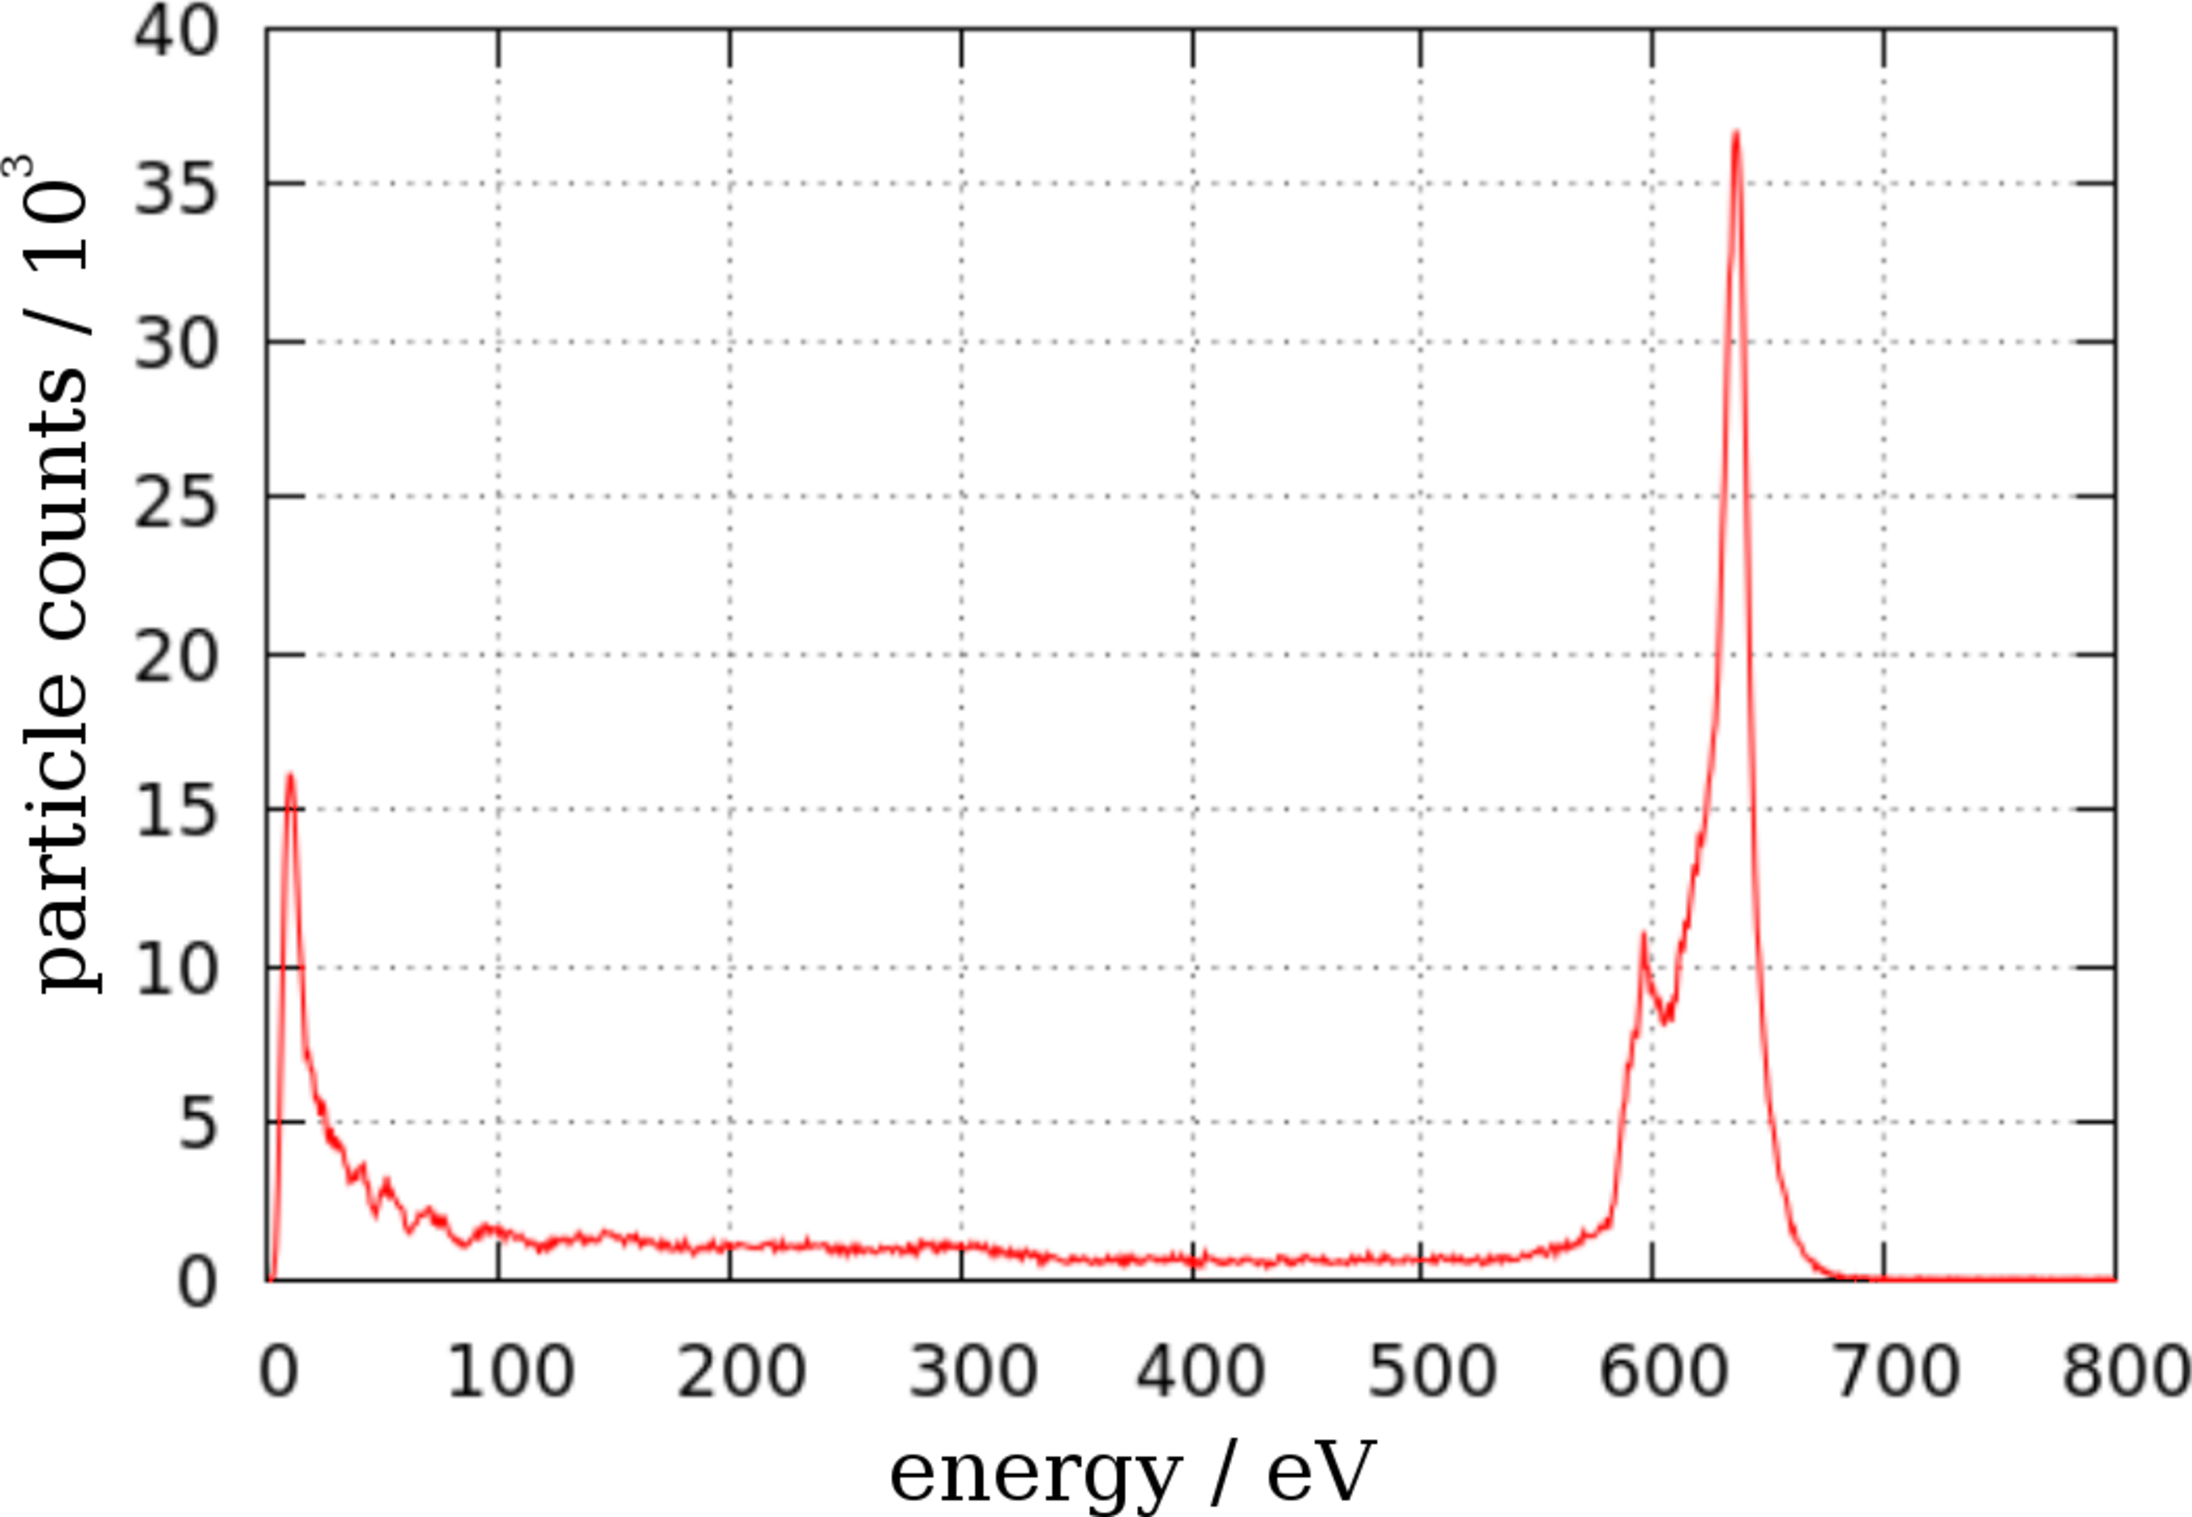
\includegraphics[width=.8\textwidth]{figures/scheuer_anionedf.pdf}
            \caption[Experimentally measured anion EDF at the anode]{%
                Experimentally measured anion energy distribution function impinging %
                on the grounded electrode. Magnesium oxide was used as cathode material, %
                which was powered with $\SI{50}{\watt}$~\cite{Scheuer15}.}
            \label{fig:anionedf_scheuer}
        \end{figure}
%
        Reactive plasmas are a common tool in many industrial and scientific applications, such as semiconductor and computer chip production. Of high importance for the surface treatment are etching and sputtering processes~\cite{Cvelbar05,Zeuner98}. Especially in electronegative discharges sputter and deposition rates are increased. They depend crucially on the distribution function of impinging ions. Therefore, a detailed understanding of these distribution functions is needed to optimise the processes. Capacitively coupled discharges with radio-frequency modulated voltages (ccrf) have high-energy ions impinging on the electrodes. Their advantage is the absence of a net current onto the target, which preserves the structure of the product.\\
        Laboratory experiments with ccrf oxygen discharges at low pressures and temperatures show a high-energy peak in the energy distribution function (EDF) of negative ions impinging on the anode. The position of this peak depends on the electrode material~\cite{Scheuer15}. Experimentally measured anion EDF is shown in~\autoref{fig:anionedf_scheuer}. A possible explanation is proposed by Stoffels and Kawano et al.~\cite{Stoffels01,Kawano83}: negative ions are produced by ionisation close to or at the surface of the electrode. The drawback of this theory is the lack of experimental or theoretical ionisation probabilities for anions at metal surfaces. Until now an explanation for this characteristic feature of the EDF of negative ions at the anode is missing.\\        
        In my thesis I will try to study this system and to improve the understanding of the underlying physics of the high-energy peak in the EDF of negative ions at a grounded electrode. Since the EDF is non-Maxwellian, a kinetic model is needed. Therefore, a Particle-in-Cell (PIC) code with Monte-Carlo-Collisions (MCC) is used to model the asymmetric ccrf discharges of low-temperature oxygen plasmas. In particular, an surface ionisation module for negative ions is introduced in the simulation and its effect on the EDF is studied.\\
        In this thesis I will try to answer the following questions:
      
        \begingroup\par
            \centering
            \bigskip\fbox{
                \parbox[c]{0.8\textwidth}{
                    \begin{enumerate}
                        \item What determines the physics of ccrf low pressure oxygen plasmas?
                        \item What is the influence of surface processes on the %
                                distribution function of negative ions?
                    \end{enumerate}
                }
            }
            \bigskip\par
        \endgroup
        
        Numerical investigations of electronegative plasmas have been done, e.g.\@ by~\cite{Matyash07oxIII,Bronold07b,Matthias15} using an one-dimensional PIC model. It has proven to be a great tool for fundamental studies of reactive radio frequency plasmas. Although this is a good approach for the investigation of axial distribution functions of plasma species close to the axis, the 1D simulations lacks effects of radial transport, asymmetry and plasma-wall interaction. For these topics, a 2D radial-axial model is needed, which is validated by comparison with the existing 1D code. In the 2D model, additional effects, such as voltage offset \emph{self bias} in ccrf discharges and asymmetry effects are taken into account.%
%        
        \par\bigskip
        To be able to answer the basic scientific question formulated before, I will firstly introduce the basic physics of plasmas in front of walls, the so-called plasma sheath. This will be extended to ccrf conditions, where the plasma reacts dynamically to the RF heating. The need for kinetic models to resolve the full distribution functions of all plasma species is satisfied by the PIC-MCC simulation method, which will be summarised shortly. As a part of the computational model, the relevant collision processes for such ccrf oxygen plasmas are discussed.\\
        In the second part of the thesis I will simulate the axial centre of the discharge without asymmetry effects using the one-dimensional model. These results are also used for a validation of the 2D radial-axial model.  After its successful validation the 2D model is used to simulate the experimental conditions of the plasma discharge from~\cite{Scheuer15}. In the PIC simulations, special emphasis lies on the investigation of surface and asymmetry effects and their impacts. Finally, the work is summarised.
%
% ************************************************************************** %
% BASICS
	%
\chapter{Physical Properties of Low Temperature RF Plasma}\label{sec:chapter_ccrfbasics}
%
	In this first chapter I will provide the necessary physical background for this work about the numerical simulation of low temperature capacitively coupled radio frequency plasma. Here both the mathematical basics and method for the simulation, as well as the most important aspects about the plasma properties will be explained.
%
	\section{Plasma Physics}\label{sec:plasmaphysics}
%
  	\subsection{Capacitively Coupled Radio Frequency Plasma}\label{sec:ccrf}
%
		The experiment where after the conducted simulations is modelled after revolves around a capacitively coupled radio frequency, low temperature plasma at low pressures of oxygen. Here, I will refer to a plasma as an globally quasi-neutral gas, consisting of freely moving charges --- e.g.\@ electrons, positively and negatively ions --- and neutral gas particles. The ratio between charged and neutral species defines the \emph{degree of ionization}, which in this case is very low. The term of global neutrality emphasizes the purpose for different length scales inside the gas itself. Hence, the associated condition of neutrality by equal densities $n\ix{e}\,=\,n\ix{i}$ only is valid for areas larger than the so called \emph{Debye sphere}. Inside this ball with a radius of $\lambda\ix{D}$ the \emph{Debye length}, the afore-mentioned neutrality is not satisfied.\\
		The creation of a plasma is accomplished by 2 parallel metal plates, the electrodes, where on at least one an ac signal at radio frequency is applied --- this kind of experimental setup is among the most common, thus being used for basic but also in-depth studies of the afore-mentioned discharges. Here, a rf signal at exactly $\SI{13.56}{\mega\hertz}$ with an amplitude between $100$--$\unit[1000]{V}$ will be used. This equals to a wavelength of $\SI{22.11}{\metre}$ for the electric field wave, which is orders of magnitude higher than the eventually simulated experiment. The use of external magnetic fields is not within the scope of this work --- correspondingly, the experiment I will refer to, also did not include any kinds of magnetic confinement or manipulation. \\
		That said, a multitude of electric setups are possible, such as coated or grounded electrodes. Therefore, different regimes of operation ensue. For example, differently driven or shaped metal plates heavily influence the charge creation process inside the plasma. In summary, the electrodes, neutral gas and electric layout resemble a dielectric hindered plate capacitor. This simplification can be used to access important physical properties, such as an additional voltage offset on one of the electrodes or charge currents at such. A basic scheme of an asymmetric rf discharge can be seen in~\autoref{fig:circuitselfbias_1}. In the case of different electrode sizes, as seen in the scheme, the potential inside the spatially restricted area between wall and discharge can change drastically. This plasma sheath forms also between grounded parts of discharge containment or probes and plasma volume. This additional direct current offset is called \emph{self-bias} (see~\autoref{sec:selfbias}). A dielectric displacement current between plasma sheath and volume accommodates as a result of the different time scales of particle movement (see~\autoref{sec:displacementcurrent}).
%
		\begin{wrapfigure}[17]{r}{0.42\textwidth}
			\centering
			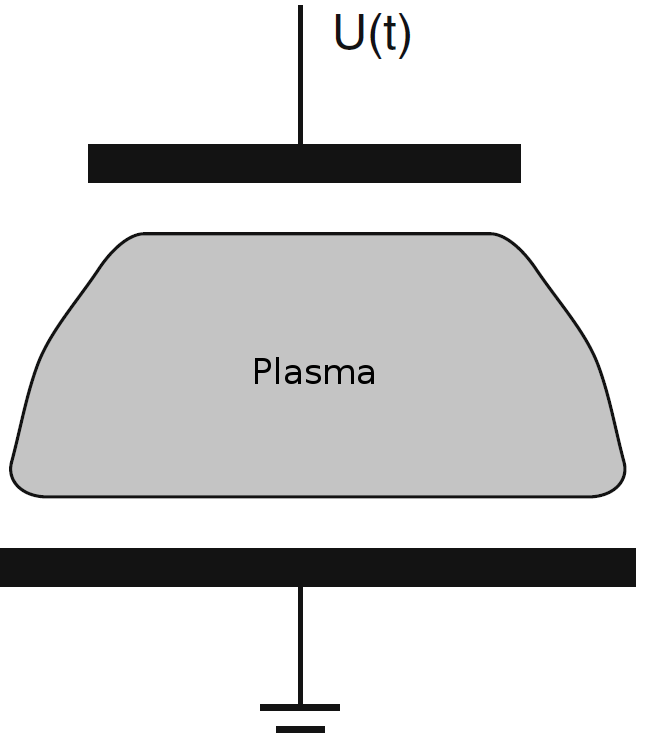
\includegraphics[width=0.38\textwidth]{figures/circuitselfbias_1.png}
			\caption{%
				Schematic of an asymmetric discharge with one grounded and %
			one driven electrode~\cite{Piel10}.}\label{fig:circuitselfbias_1}
		\end{wrapfigure}
%
		Especially, self-bias and displacement current play a key role in the following investigations, as a capacitive coupling between electrodes and power supply is difficult to model in a numerical kinetic simulation.	A strong mathematical analysis of general plasma properties would not be suitable for this kind of work, although certain aspects will be discussed later, such as in~\autoref{sec:selfbias} and~\autoref{sec:displacementcurrent}.	In comparison to other low temperature, low pressure discharges  --- an example could be a dielectric hindered dc discharge at high voltages, with an electrode space gap of just a couple millimeters ---, radio frequency plasma are characterized by their unique transport process inside the sheath and heating mechanisms of charged species. A more in-depth discussion can be found in~\autoref{sec:heating}.

	%
		\section{Plasma-Wall Interaction}\label{sec:sheathphysics}
%
%       !!! DIESER GANZE ABSCHNITT GEHÖRT IN DEN TEIL VORHER INTEGRIERT, 
%           SO DASS MAN DA DIE SCHICHT WIRKLICH VERSTEHEN KANN !!!
%           LOGIK:1) SCHICHT 2) CCRF-EFFEKTE
%
            In contrast to the plasma bulk, the charge densities do not satisfy the quasi-neutrality condition in a distance of $d$ from the wall. Because of the negative potential around a wall the transport processes of electrons and ions are perturbed. The potential barrier reflects electrons of low kinetic energies, although both particle species diffuse into the sheath. Because continuity has to be satisfied, e.g\@ $j\ix{e}=j\ix{i}$ at the sheath-boundary, negative space charges build up and the corresponding electric fields accelerate the ions to match this condition.\\
            The physicals law which characterise those transport processes are derived in the following sections. 
%
			\subsection{Child-Langmuir Law}\label{sec:langmuirlaw}
%			
				\begin{wrapfigure}[18]{r}{0.5\textwidth}
					\centering%
					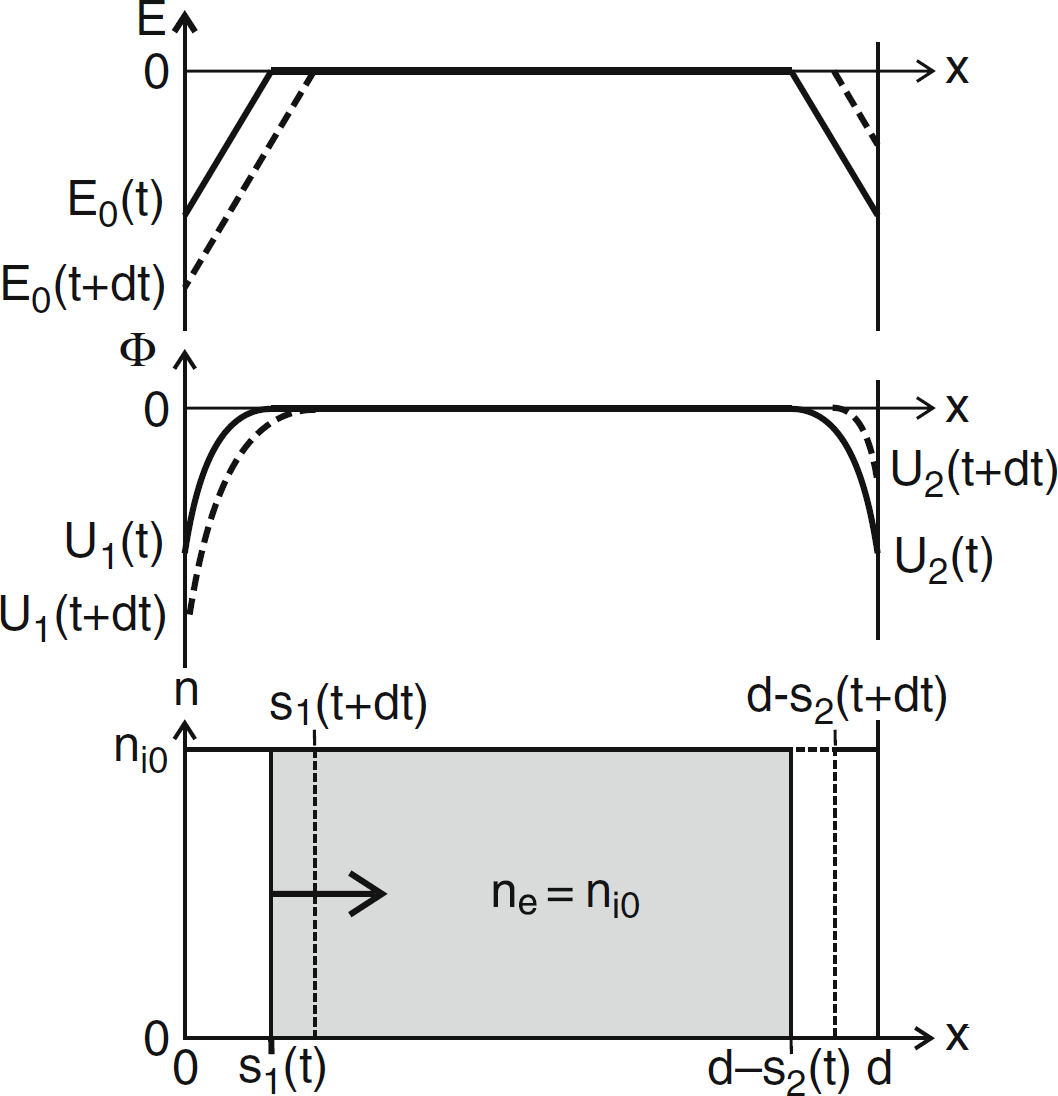
\includegraphics[width=0.45\textwidth]{figures/displacement_current_piel.png}%
					\caption{%
						One dimensional density, potential and electric field for an asymmetric, harmonically %
						driven discharge.~\cite{Piel10}}\label{fig:displacementcurrent}
				\end{wrapfigure}
%
			In an one-dimensional model, a negatively charged wall at $x=0$ creates a potential barrier for electrons of thermal velocity, e.g.\@ $|\Phi(0)-\Phi(d)|\ll k\ix{B}T\ix{e}/e\,$. The thickness of the space-charge sheath here is $d$ and the sheath-boundary therefore at $x=-d$ (see~\autoref{fig:sheath_piel}). It is usually the size of a few Debye-length $\lambda\ix{D}$. The electron density $n\ix{e}(x)$ towards the wall can be written with a \emph{Boltzmann} distribution function $f\ix{B}(\Phi)\sim\exp(e\Delta\Phi/k\ix{B}T\ix{e})\,$~\cite{Piel10}. This means that the electron density decreases exponentially towards the negatively charged wall.\\
			It can be assumed that the sheath thickness $d\ll s\ix{mfp,i}$ the mean free path of the ions inside the plasma bulk. Hence the ions enter the pre-sheath collisionless at a speed $v\ix{i,0}$. The ion and electron densities are therefore:
%
				\begin{align}
					n\ix{i}(x)=n\ix{i}(d&){\left(1-\frac{2e\Phi(x)}%
						{m\ix{i}v\ix{i,0}^{2}}\right)}^{-1/2}%
%						\nonumber\\[0.2cm]%
						\quad\text{~and~}\quad
						n\ix{e}=n\ix{e}(d)\exp&\left(%
						\frac{e(\Phi(x)-\Phi(d))}{k\ix{B}T\ix{e}}\right)\,%
						\label{equ:ionandelectrondens}
				\end{align}
%
			At the boundary between bulk and pre-sheath, the walls potential vanishes because of the plasmas shielding capabilities. Furthermore, one can assume that the kinetic energy of the ions at this point is smaller than the potential energy for the acceleration inside the pre-sheath, e.g.\@ $m\ix{i}v\ix{i,0}^{2}\ll |e\Phi(x)|$. Using \emph{Poisson's} equation gives an expression for the potential $\Phi(x)$ Solving this, and using the unperturbed ion current $j\ix{i}=n\ix{i}(d)ev\ix{i,0}$, one yields the result by \emph{Langmuir} in~\autoref{equ:langmuirpot}:
%
				\begin{align}
					\Delta\Phi\cong-\frac{en\ix{i}{\left(-d\right)}%
						}{\varepsilon\ix{0}}{\left(-\frac{2e\Phi{%
						\left(x\right)}}{m\ix{i}v\ix{i,0}^2}\right)}^{-\frac{1}{2}}%
					\quad\Rightarrow\quad%
					\Phi{\left(x\right)}=&{\left({\left(\frac{3}{4}{\left(x+d%
						\right)}\right)}^4{\left(\frac{j\ix{i}}{\varepsilon\ix{0}%
						}\right)}^2\frac{m\ix{i}}{2e}\right)}^{\frac{1}{3}}%
						\label{equ:langmuirpot}
				\end{align}
%
				Solving again for $j\ix{i}$ yields the \emph{Child-Langmuir Law} (see~\autoref{equ:childlangmuirlaw}). This equation defines the ion current as a function of the unperturbed plasma bulk. In other words, the sheath changes its thickness in dependency of the discharge parameters, always satisfying the ion current defined by the Child-Langmuir Law:
%
				\begin{align}
					j\ix{i}=\frac{4}{9}&\varepsilon\ix{0}{\left(\frac{2e{%
						\left(\Phi{\left(-d\right)}-\Phi{\left(0\right)}%
						\right)}^3}{m\ix{i}d^2}\right)}^{\frac{1}{2}}%
				    	\label{equ:childlangmuirlaw}
				\end{align}
%				
				The \emph{Child-Langmuir Law} yields an expression for the relation between potential and current on a wall in a space-charge limited plasma region, e.g\@ the sheath. It characterises transport processes between a floating wall and the plasma bulk. Therefore it is important to understand, for example the oscillation of the sheath boundary in rf plasmas or secondary emission processes at walls.
	%
		\subsection{Bohm Criteria}\label{sec:bohmcriteria}
%
			In~\autoref{sec:sheathphysics} the behaviour of charge particle densities inside the plasma sheath has been discussed. In contrast to the discharge volume, those densities do not satisfy the quasi-neutrality condition in a distance of $d$ from the wall any more. Though we know that the sheath is a spatially restricted area around electrostatic floating surfaces, a physical law concerning this circumstance has not been derived here. So the question ensues, why the area of electron depletion does not extend further into the discharge volume.\\
			To answer this question, one has to take a look at a substitutional system. This will be a, likewise mechanical, one-body extremal problem of a point mass. In this case only kinematic potentials with inverted parabolic maxima are of interest. Therefore, in this unstable equilibrium, a small pertubation culminates into a large force on the test body.\\
			To see the quality of this example, one has to take a look at the second order differential equation of the afore-mentioned mechanical problem and the electrostatic \emph{Poisson's equation} (see~\autoref{equ:pseudo}).
%
			\begin{align} 
				m\frac{\diff^{2}\vec{r}}{\diff t^{2}}=-\frac{\diff V}{\diff\vec{r}}%
						\quad\Leftrightarrow\quad%
						\Delta_{\vec{r}}\Phi=-\frac{\diff\Psi}{\diff\Phi}=f{\left(\Phi\right)}%
						\hspace{-0.33cm}\overset{\text{Poisson's}}{\overset{\mid}{=}}\hspace{-0.33cm}%
						\frac{\rho}{\varepsilon\ix{0}}%
				\label{equ:pseudo}
			\end{align}
%
			\begin{figure}[!b]
				\centering%
				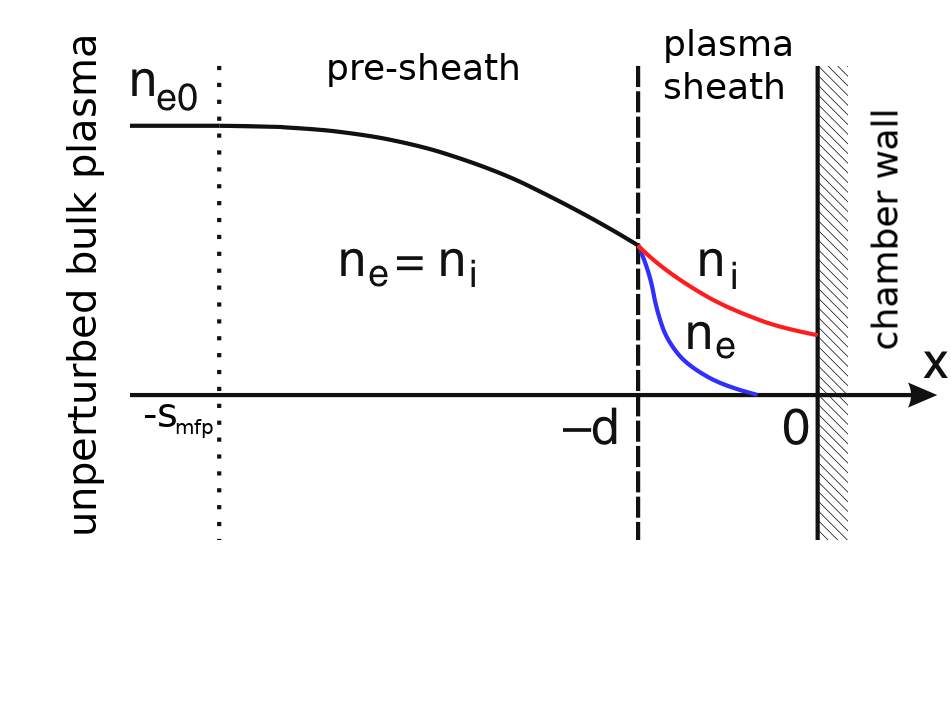
\includegraphics[width=0.6\textwidth]{figures/sheath_piel.png}%
				\caption{%
				One dimensional density profiles as a function of the distance to a floating wall. Note the exponential decrease of the electron density $n\ix{e}$ from the sheath border towards the presumably negatively charged wall. Densities allready reach approximately $0,66n\ix{e,0}$ inside the pre-sheath.~\cite{Piel10}}\label{fig:sheath_piel}
			\end{figure}
%
			For an instability, the force on the test body must increase with the distance from the equilibrium, hence the~\autoref{equ:inequality} is used to calculate the exact velocity at which an ion is entering the sheath. This results in the first \emph{Bohm criteria}.
%
			\begin{align}
				0>\left.\frac{\diff^{2}\Psi}{\diff\Phi^{2}}\right|_{\Phi=0}%
				\overset{\text{\autoref{equ:pseudo}}}{\overset{\mid}{=}}%
						\left.\frac{\diff}{\diff\Phi}\left(\frac{n\ix{e}\left(x\right)-n\ix{i}%
						\left(x\right)}{\varepsilon\ix{0}}\right)\right|_{\Phi=0}&%
						\frac{en\ix{e}\left(-d\right)}{\varepsilon\ix{0}}\left(\frac{e}%
						{k\ix{b}T\ix{e}}-\frac{e}{m\ix{i}v\ix{i,0}^{2}}\right)%
				\label{equ:condition}\\[10pt]%
				\Rightarrow\quad%
				v\ix{i,0}\ge v\ix{i,B}=\sqrt{\frac{k\ix{B}T\ix{e}}{m\ix{i}}}&%
				\label{equ:inequality}
			\end{align}
%	
			Analoguos you can define the so called \emph{Mach number} $M=v\ix{i,0}/v\ix{i,B}$, where $v\ix{i,B}$ denotes the \emph{Bohm velocity}.\\
			Now, to understand why the sheath does not extend further than a fixed distance $d$ from the discharge boundary, the particle movement has to be investigated on a smaller scale. As seen above, there is an electric field in the \emph{pre-sheath} that accelerates the ions to $v\ix{i,B}$. In addition, quasi-neutrality is still satisfied here:
%
			\begin{align}
				n\ix{i}\left(x\right)=n\ix{i,0}\exp\left(\frac{e\Phi\left(x\right)}{k\ix{B}T\ix{e}}\right)%
				=n\ix{e}\left(x\right)\,\,.%
				\label{equ:quasineutral}
			\end{align}
%
			Still, $\Phi{\left(x\right)}$ is the potential inside the pre-sheath from~\autoref{sec:sheathphysics} and $n\ix{i,0}$ the unperturbed density from the plasma \emph{bulk}. A greater part of the ion transport process in this area is governed by collisions with neutral gas particles, hence the velocity distribution function with the collision frequency $\nu\ix{n,i}$ has to be rewritten:
%
			\begin{align}
				\frac{\diff v\ix{i}}{\diff x}=\frac{\nu\ix{n,i}v\ix{i}^{2}}{v\ix{B}^{2}-v\ix{i}^{2}}\quad.%
				\label{equ:distribution}
			\end{align}
%
			From the singularity in~\autoref{equ:distribution} at $v\ix{i}=v\ix{B}$ and the knowledge of $\Phi(x)$ at the wall, one can calculate the sheath thickness $d$. Furthermore, ions with velocities smaller than the Bohm velocity are being accelerated inside the pre sheath. According to~\autoref{equ:inequality} velocities greater than $v\ix{B}$ are not allowed here. This is, together with~\autoref{equ:distribution} the reason why the ion velocity is exactly $v\ix{B}$ at the boundary of the plasma sheath and thus a positive space-charge ensues.
%
			\begin{align}
				M\ge1%
				\Leftrightarrow%
				v\ix{i}(-d)\ge v\ix{B}%
				\label{equ:bohmcriteria2}
			\end{align}
%
			Conclusively, at the sheath boundary~\autoref{equ:bohmcriteria2} is satisfied.\\
			At $x=-d$, both negative and positive charge density decreased to $n\ix{i}=n\ix{e}\approx\SI{0.66}n\ix{e,0}$ (see~\autoref{fig:sheath_piel}), where the potential is approximately $-k\ix{B}T\ix{e}/2e$ because of the currents onto the wall.\\
			In summarization, the plasma does not `see' its sheath, because the ion dynamic discussed before is spatially restricted. The sheath only develops where there is electron depletion or an externally applied, negative potential.

	%
			\subsection{Surface Effects}\label{sec:surfaceeffects}
%			
			Although the sheath physics are influenced by plasma properties in front of the wall, such as temperatures and densities, they are also sensitive to wall processes. One important aspect is the absorption and re-emission of ions and electrons.
%				
			\paragraph{Secondary Electron Emission}
			If fast electrons impact on a wall, there is a chance for them to collide with electrons of the solid and to release secondary electrons from the surface. The \emph{secondary electron emission} coefficient is defined as $\gamma$: one impinging electron emits $\gamma$ electrons from the metal. This \emph{SEE} reduces the $\Delta\Phi$ of the sheath potential because it creates an additional electron current from the wall towards the sheath edge, therefore altering the continuity condition $j\ix{i}=j\ix{e}$. A new \emph{effective potential drop} $\Delta\Phi\ix{eff}$ can be derived in~\autoref{equ:effectivepotentialdrop}. There is a critical value $\gamma\ix{c}$ where the wall potential gets unstable~\cite{Duras11}.
%
				\begin{align}
					\Delta\Phi\ix{eff}=-\frac{k\ix{B}T\ix{e}}{e}\cdot\ln\left(\left(1-%
							\gamma\right)\sqrt{\frac{m\ix{i}}{2\pi m\ix{e}}}\,\right)%
					\label{equ:effectivepotentialdrop}
				\end{align}
%
				\paragraph{Secondary Ion Emission}	
				Experimental results from~\cite{Kullig12} indicate that ions are produced near the surface of a metal electrode and heavily accelerated in the plasma sheath. In theory, secondary emission by surface ionisation --- in analogy to the surface neutralisation --- occurs with incident atoms of thermal energy. Hence one assumes a positively biased wall at high temperatures as the target. Its valence level is therefore broadened, giving an atom $A$ the chance to deposit an electron at the metal. After reaching thermal equilibrium, a positive ion can be emitted by chance. This statistical process can be described by a thermodynamic equation (see~\autoref{equ:sahalangmuirpos}) yielding the ionisation coefficient of $A$. In~\autoref{equ:sahalangmuirpos} a modified approach for the \emph{Saha-Langmuir equation} on the degree of ionisation in gases can be found. Here, the surface temperature $T$ and average work function $\overline{\Phi}_{+}$ are important quantities.	Additionally, the ionization energy $I(A)$ --- or impact energy ---, the particle fluxes of both species $j$ and $j^{+}$, corresponding statistical weights $w$, $w^{+}$ and reflection coefficients at the intrinsic potential barrier $r$/$r^{r}$ are used.
%
				\begin{align}
					A\leftrightharpoons A^{+}+&\,e^{-}%
					\nonumber\\[0.0cm]
					\alpha^{+}(A^{+})=\frac{j^{+}}{j}=\frac{(1-r^{+})\,w^{+}}{(1-r)\,w}\cdot&\exp\left(%
					\frac{\overline{\Phi}_{+}+e\sqrt{eV\ix{ext}}-I(A)}{k\ix{B}T}\right)%
					\label{equ:sahalangmuirpos}
				\end{align}
%
				The \emph{Schottky term} $e\sqrt{eV\ix{ext}}$ describes the reduction of the work function of electrons in a metal solid due to a large external electric field. At high temperatures of, e.g.\@ $\unit[1000]{K}$ and applied voltages $V\ix{ext}<\unit[1]{kV}$, this term and the corresponding internal reflection coefficients $r$/$r^{+}$ can be neglected --- it appears to be just half of the thermal energy at room temperature. However, theoretical studies for such coefficients are missing.\\
				In addition to SIE of positive ions, the model can be easily applied for negative ions with small changes to~\autoref{equ:sahalangmuirpos}: a negatively biased electrode is assumed and the average work function yields a different sign. The electron affinity of the incident particle $B$ is $A(B)$.
%
				\begin{align}
					B+\,&e^{-}\leftrightharpoons B^{-}%
					\nonumber\\[0.2cm]
					\alpha^{-}(B^{-})=\frac{(1-r^{-})%
						\,w^{-}}{(1-r)\,w}\cdot&\exp\left(%
						\frac{-\overline{\Phi}_{-}+e\sqrt{eV\ix{ext}}+A(B)}{k\ix{B}T}\right)%
					\label{equ:sahalangmuirneg}
				\end{align}
%
				Applying the former assumptions to both equations of positive and negative ions, inserting a homogeneous work function $\Phi=\overline{\Phi}_{-}=\overline{\Phi}\ix{+}$ for the used substrate yields the originally derived \emph{Saha-Langmuir equations}.
%				
				\begin{align}
					\alpha^{+}(A^{+})=\frac{w^{+}}{w}\,\exp\left(\frac{%
					\Phi-I(A)}{k\ix{B}T}\right)\,,%
						\quad\quad%
					\alpha^{-}(B^{-})=\frac{w^{-}}{w}\,\exp\left(\frac{%
						-\Phi+A(B)}{k\ix{B}T}\right)%
						\label{equ:sahalangmuirshort}
				\end{align}
%
				Though only considering atomic particles onto the wall, forms similar to~\autoref{equ:sahalangmuirshort} can also be derived for molecular surface interactions~\cite{Kawano83}. For conditions and materials of ccrf discharges no calculated reflection coefficients.\\
				Works of, e.g.\@~\cite{Ustaze97} and~\cite{Los90} investigated ion beam scattering, electron loss and transport in plasma sheath environments for metal walls, especially $\text{MgO}(100)$ surfaces. There Ustaze et al.~\cite{Ustaze97} studied incident oxygen gas particles --- ions and neutrals ---  on magnesium oxyde surfaces. Impinging atoms became negatively charged ions, picking up electrons from the $\text{MgO}$ of the wall. This interaction, though requiring a minimum ionization and liberation energy for the electron, is most effective at low energies $<\unit[1]{eV}\,$. This is due to a maximum of residence time at the target for an incoming atom. Hence it can be considered a non-resonant charge transfer process at the anion site. Further details can be found in~\cite{Kawano83}.\\
				Ions hitting onto the wall will result in an anion current in opposing direction:
%
				\begin{align}
					j_{-}=\eta\,j\ix{+}\,\,,%
					\label{equ:negative_efficiency}
				\end{align}
%
				with a corresponding efficiency of an incident positive particle $\eta\,$. The same stability criteria apply for $\eta$ as they do for the electron emission coefficient $\gamma$. In case of SIE beyond a critical value $\eta\ix{c}$, a second plasma sheath may develop, enclosing the bulk and an inner sheath and reducing transport in-between.
	%			\begin{wrapfigure}[13]{r}{0.4\textwidth}
%				\centering%
%				\vspace*{-0.5cm}%
%				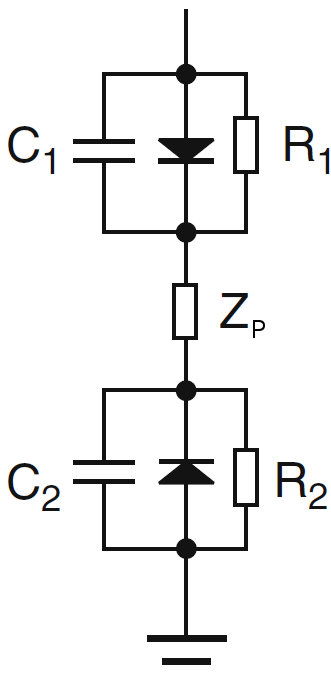
\includegraphics[width=0.17\textwidth]{figures/circuit_selfbias_piel.png}
%				\caption{%
%					Replacement circuit of an asymmetrically driven ccrf %
%					discharge.~\cite{Piel10} A diode represents the directed electron %
%					current from the sheaths $j=1,2$.}\label{fig:replacementcurrent}
%			\end{wrapfigure}
%
%           A step towards the characterisation of asymmetric ccrf discharges is the development of a replacement circuit, see~\autoref{fig:replacementcurrent}. Thus, one can define a specific impedance for a rf discharge of excitation frequency $\omega$. The value of $\varepsilon\ix{p}$ resembles the permeability of the working gas between the driven and/or grounded electrode~\cite{Piel10}. In addition, this volume has the capacity $C\ix{p}$ --- the capacity of a cubicle with a cross section $A$, thickness $b$ and electron-neutral collision frequency $\nu\ix{e,n}$ calculates like~\autoref{equ:capacityandepsilon}.
%
%				\begin{align}
%					\varepsilon\ix{p}=&1-\frac{\omega\ix{p,e}^2}{\omega\left(\omega-\imag\nu\ix{e,n}\right)}\,,%
%						\quad\quad%
%						C\ix{p}=\varepsilon\ix{p}C\ix{0}=%
%						\varepsilon\ix{p}\varepsilon\ix{0}\frac{A}{b}%
%						\label{equ:capacityandepsilon}\\[0.2cm]
%					&Z\ix{p}={\left(\imag\omega C\ix{p}+ \frac{1}{\frac{1}{\omega\ix{p,e}^2C\ix{0}}%
%							{\left(\nu\ix{e,n}+\imag\omega\right)}}\right)}^{-1}%
%					\label{equ:bulkimpedanz}
%				\end{align}
%		
%				The~\autoref{equ:bulkimpedanz} represents the full electrical impedance, consisting of the inverse sum of real and imaginary resistance, as well as the capacity of the neutral gas volume. Here, $\imag\omega/(\omega\ix{p,e}^{2}C\ix{0})$ characterizes the electrons inertia in regard to an external excitation $\omega$. The real part $\nu\ix{e,n}/(\omega\ix{p,e}^{2}C\ix{0})$ denotes the resistance by neutral particle collisions. For high excitation frequencies, e.g.\@ $\SI{13.56}{\mega\hertz}$ the bulk impedance can be neglected (see~\autoref{equ:bulkimpedanz}~\cite{Kay85}). Both sheath capacities of anode and cathode take the dominant part.
%
%				If the excitation frequency $\omega$ is small compared to other time scales, e.g\@ electron and ion plasma frequencies, the electron current from the sheath becomes bigger than the displacement current. Hence the electron current onto the driven electrode decreases by a Maxwell factor --- this is a function of the there-on applied voltage --- compared to the corresponding ion current. Therefore the sheaths impedance is bigger than those of the floating walls. Together with~\autoref{equ:selfbias_1} and~\autoref{equ:inequality} the plasma potential $\Phi\ix{p}$ vanishes and only the currents onto the driven electrode have to be equal. With $\mathbf{I}\ix{0}$ the zeroth order modified \emph{Bessel function} the following equation yields the self bias voltage:
%      
%				\begin{align}
%					U\ix{sb}=\frac{k\ix{B}T\ix{e}}{e}\ln%
%						\left[\mathbf{I}\ix{0}\left(\frac{eU\ix{rf}}{k\ix{B}T\ix{e}}\right)\right]\,.%
%					\label{equ:selfbias_3}
%				\end{align}
%
        \section{Asymmetric Capacitively Coupled RF Discharges}\label{sec:selfbias}
%   
           Most rf plasmas are asymmetric discharges due to the contact of the ionised gas with the vacuum vessel. The asymmetry is characterised by the area ratio of driven electrodes and grounded walls. The faster and more mobile electrons create a potential bias on the driven electrodes. If those are capacitively coupled to the driver, there can not be any net current over one rf cycle. The accumulated charge can not be flushed and the \emph{self bias} establishes to satisfy continuity.\\
				First, let us assume the plasma potential $\Phi\ix{p}(t)$ and voltage across the discharge $U(t)$ to be:
%
				\begin{align}
					U\left(t\right)=U\ix{sb}+U\ix{rf}\sin\left(\omega t\right)%
%						\nonumber\\[0.0cm]
						\quad\text{~and~}\quad%
						\Phi\ix{p}\left(t\right)=\overline{\Phi\ix{p}}+%
						\Phi\ix{rf}\sin\left(\omega t\right)\,.%
						\label{equ:selfbias_1}
				\end{align}
%
			    A common approximation for the self bias voltage is roughly half of the driven electrodes peak-to-peak voltage: $|U\ix{sb}|\approx U\ix{rf}/2$. \\
			    Both sheaths of the electrodes collapse completely during a full cycle of $U(t)$. At this moment, no potential barrier or space charge is hindering the particles to hit the electrodes. Electrons and ions can impinge on the surface and force the plasma potential $\Phi\ix{P}$ to level out with the walls. This short circuit between plasma and sheath occurs when $\Phi\ix{P}$ becomes negative with regard to the excitation ---~\autoref{equ:selfbias_unequal} and~\autoref{fig:circuitselfbias_2} express this circumstance:
%
				\begin{align}
					\Phi_{\text{p},\max}=\overline{\Phi\ix{p}}+\Phi\ix{rf}\geq U\ix{sb}+U\ix{rf}\,,%
%						\nonumber\\[0.0cm]
						\quad\quad%
						\Phi_{\text{p},\min}=\overline{\Phi\ix{p}}-\Phi\ix{rf}\geq0%
						\label{equ:selfbias_unequal}
				\end{align}
%
				\begin{figure}[!t]
					\centering%
					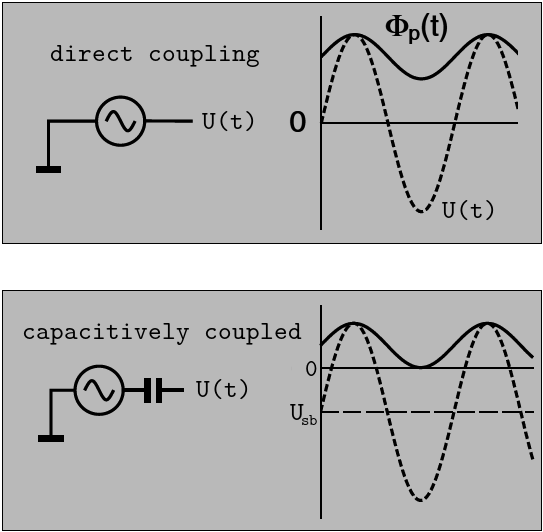
\includegraphics[width=0.95\textwidth]{figures/selfbiasvoltage.png}
					\caption{%
						Schematics of the voltage $U(t)$ and plasma potential $\Phi(t)$ %
						for a directly and capacitively coupled rf discharge. Different cases of %
						symmetry are shown: enlarged driven electron, grounded %
						electrode and a symmetric discharge.~\cite{Piel10}}\label{fig:circuitselfbias_2}
				\end{figure}
%
				If there is no special coupling between electrode and electrical driver, the equality in~\autoref{equ:selfbias_unequal} is true. However, if a capacitive coupling is used, there can not be any net current between excitation and electrode because of charge conservation and current continutiy. The capacitance can not be inverted over the course of one rf cycle. The electron currents are then equal on both electrodes, therefore shifting the minimum plasma potential to ground and the maximum to the excitation. The dc \emph{self bias} part $U\ix{sb}$ and the mean plasma potential $\overline{\Phi\ix{p}}$ become:
%
				\begin{align}
					\overline{\Phi\ix{p}}=\frac{1}{2}(U\ix{sb}+U\ix{rf})%
%					    \nonumber\\[0.0cm]
                        \quad\text{~and~}\quad%
    					U\ix{sb}=\frac{C\ix{1}-C\ix{2}}{C\ix{1}+C\ix{2}}U\ix{rf}%
						\,,%
					\label{eq:selfbiaszwei} 
				\end{align}
%
                where $C\ix{1,2}=\varepsilon\ix{p}\varepsilon\ix{0}\frac{A}{b}$ are the capacities of the corresponding plasma sheath. Here, $A$ and $b$ are cross section and thickness of the space charge volume, and $\varepsilon\ix{p}$ denotes the permeability of the working gas. Hence the value of the self bias becomes a function of discharge geometry, working gas and plasma sheath. For example, larger ratios of asymmetry, e.g.\@ $C\ix{1}\gg C\ix{2}$ lead to large values of $U\ix{sb}$.
	%			
			\subsection{Dielectric Displacement Current}\label{sec:displacementcurrent}
%
				Due to their higher mobility and plasma frequency $\omega\ix{p,e}$, the electron distribution can follow an external excitation with a similarly high frequency much better than the heavier ions species. Because of that, one can assume those as nearly stationary, e.g.\@ $\omega\ix{p,i}\ll\omega\ix{p,e},\,\omega\ix{rf}\,$. Investigating the circumstances and consequences of this relation yields the displacement current $j\ix{d}$. \\
				Let us suppose an area of thickness $d$ in front of a negatively charged wall, where the electron ensity is negligible and the corresponding ion property constant at $n\ix{0,i}$. Thus an electric field of
%   	 
				\begin{align}
					E\ix{0}=-en\ix{0,i}d/\varepsilon\ix{0}
				\end{align}
%
				establishes. If the wall potential now decreases due to electron bombardment or external manipulation, the sheaths border moves further inside into the discharges volume with the velocity $u\ix{s}=\diff s\ix{1}/\diff t$. Thus, the sheath expansion and hence charge movement creates an additional \emph{displacement current} $j\ix{d}$, which is compensated with $j\ix{d,e}$ the electron current from this border displacement. Hence charge conservation and continuity is satisfied~\cite{Godyak90a}.
%
				\begin{align}
					j\ix{d}=-en\ix{0,i}u\ix{s}=-j\ix{d,e}
				\end{align}
%
				Electrons that are pushed out of this positive space-charge area then contribute to the plasma bulk density and to the quasi neutrality $n\ix{e}=n\ix{0,i}\,$. But in case of a harmonically driven discharge, the sheath in front of the opposing electrode is shrinking with $\diff s\ix{1}=-\diff s\ix{2}\,$. Hence the spatial expansion and position of the bulk are oscillating sinusoidal, or: the sheaths thickness oscillates harmonically around a mean value, e.g\@ $s\ix{0}$. The associated voltage drop across the discharge~\cite{Piel10} between the sheath potentials $U\ix{1/2}$ is
%
				\begin{align}
					\Delta U=U\ix{1}-U\ix{2}=-\frac{2en\ix{i,0}s\ix{0}}%
						{\varepsilon\ix{0}}\exp\left(\imag\omega t\right)
				\end{align}
	%
		\subsection{Heating Mechanisms}\label{sec:heating}
%
		\paragraph{Ohmic Heating}
		In a spatially uniform electric field that oscillates harmonically perpendicular to the electrodes, as is the case in the bulk of a ccrf discharge, electrons periodically gain and lose energy in the absence of collisions without any net energy gain~\cite{Schulze09}. This is due to the symmetrical de-/acceleration in the sheaths over one rf cycle. Let us assume the electric field to have no or a negligible component parallel to the electrodes. Hence the mean absorbed power by the electrons in an oscillating electric field is
%
		\begin{align}
			\overline{P}\ix{ohm}=\omega\ix{rf}\int_{0}^{T\ix{rf}}\,j\ix{tot}(t)\cdot E(t)\diff t%
			\label{equ:meanpowerheat}\\[0.0cm]%
			%m\ix{e}\frac{\diff v\ix{e}}{\diff t}=-eE(t)-m\ix{e}\nu\ix{n,e}v\ix{e}%
			%\label{equ:heatingmotion}
		\end{align}
%
		Here $j\ix{tot}$ is the total charge current density. The total mean power dissipated into the electron species through acceleration in a harmonically oscillating electric field and neutral gas friction becomes
%
		\begin{align}
			\overline{P}\ix{ohm}=\frac{|E\ix{0}|^{2}\Re(\sigma\ix{p})}{2}=%
			\frac{|j\ix{0}|^{2}}{2\Re(\sigma\ix{p})}\,,%
			\quad\quad%
			\sigma\ix{p}=\frac{n\ix{e}e^{2}}{m\ix{e}(\nu\ix{n,e}+\imag\omega\ix{p})}%
			\label{equ:ohmicheating}
		\end{align}
%
		The property $\sigma\ix{p}$ is the plasma conductivity, hence resulting in $j\ix{0}=\sigma\ix{p}E$. This demonstrates that power from an spatially uniform, harmonically oscillating electric field can only be transferred via collisions --- the power is zero, if collisions are zero. Elastic electron-neutral collisions transfer energy into a direction perpendicular to the field. This component is not lost during the reversal of $E(t)$. Therefore the electron species gains energy during the field oscillation. This mechanism is called \emph{ohmic heating} and takes place mainly in the plasma bulk.
%
		\paragraph{Stochastic Heating}
		Low-pressure, capacitively coupled rf plasmas can be stabilised by collisionless heating in the sinusoidal modulated discharge sheaths. We will assume a `hard wall' approximation (HWA), where the electrons are considered to collide elastically with the oscillating sheath edge. Heating power is then averaged by reverse and forward energy fluxes into and out of the sheath respectively. This gives an easy access to heating mechanisms of the proposed discharges.\\
		The heating mechanism in such low pressure plasma is of particular importance, because collisions are rare and sheath processes are key to the sustainability of the discharge (see e.g\@~\autoref{sec:bohmcriteria}). This process, though relying on enough randomisation in phase-space inside the bulk, sufficiently creates a net heating of the plasma~\cite{Gozadinos01b,Goedde88}. This is referred to as \emph{stochastic heating}.\\

%		
%		\begin{align}
%			\tau\ix{n}\approx\frac{2\alpha(\mu\ix{n}-\beta%
%				\cos\varphi\ix{n})}{1+\alpha\beta\cos\varphi\ix{n}}\,,%
%			\quad\quad%
%			\mu\ix{n+1}=-\mu+\frac{2(\mu\ix{n}-\beta\sin\varphi\ix{n})}{1+\alpha\beta\cos\varphi\ix{n}}%
%			\label{equ:transitandvelocityheating}
%		\end{align}
%
%		In \emph{hamiltonian mappings}, those two variables are not canonically conjugate, hence insufficient for checking conserved quantities. One has to keep that in mind when evaluating the HWA approximation.
%
		\begin{figure}[!t]
			\centering
			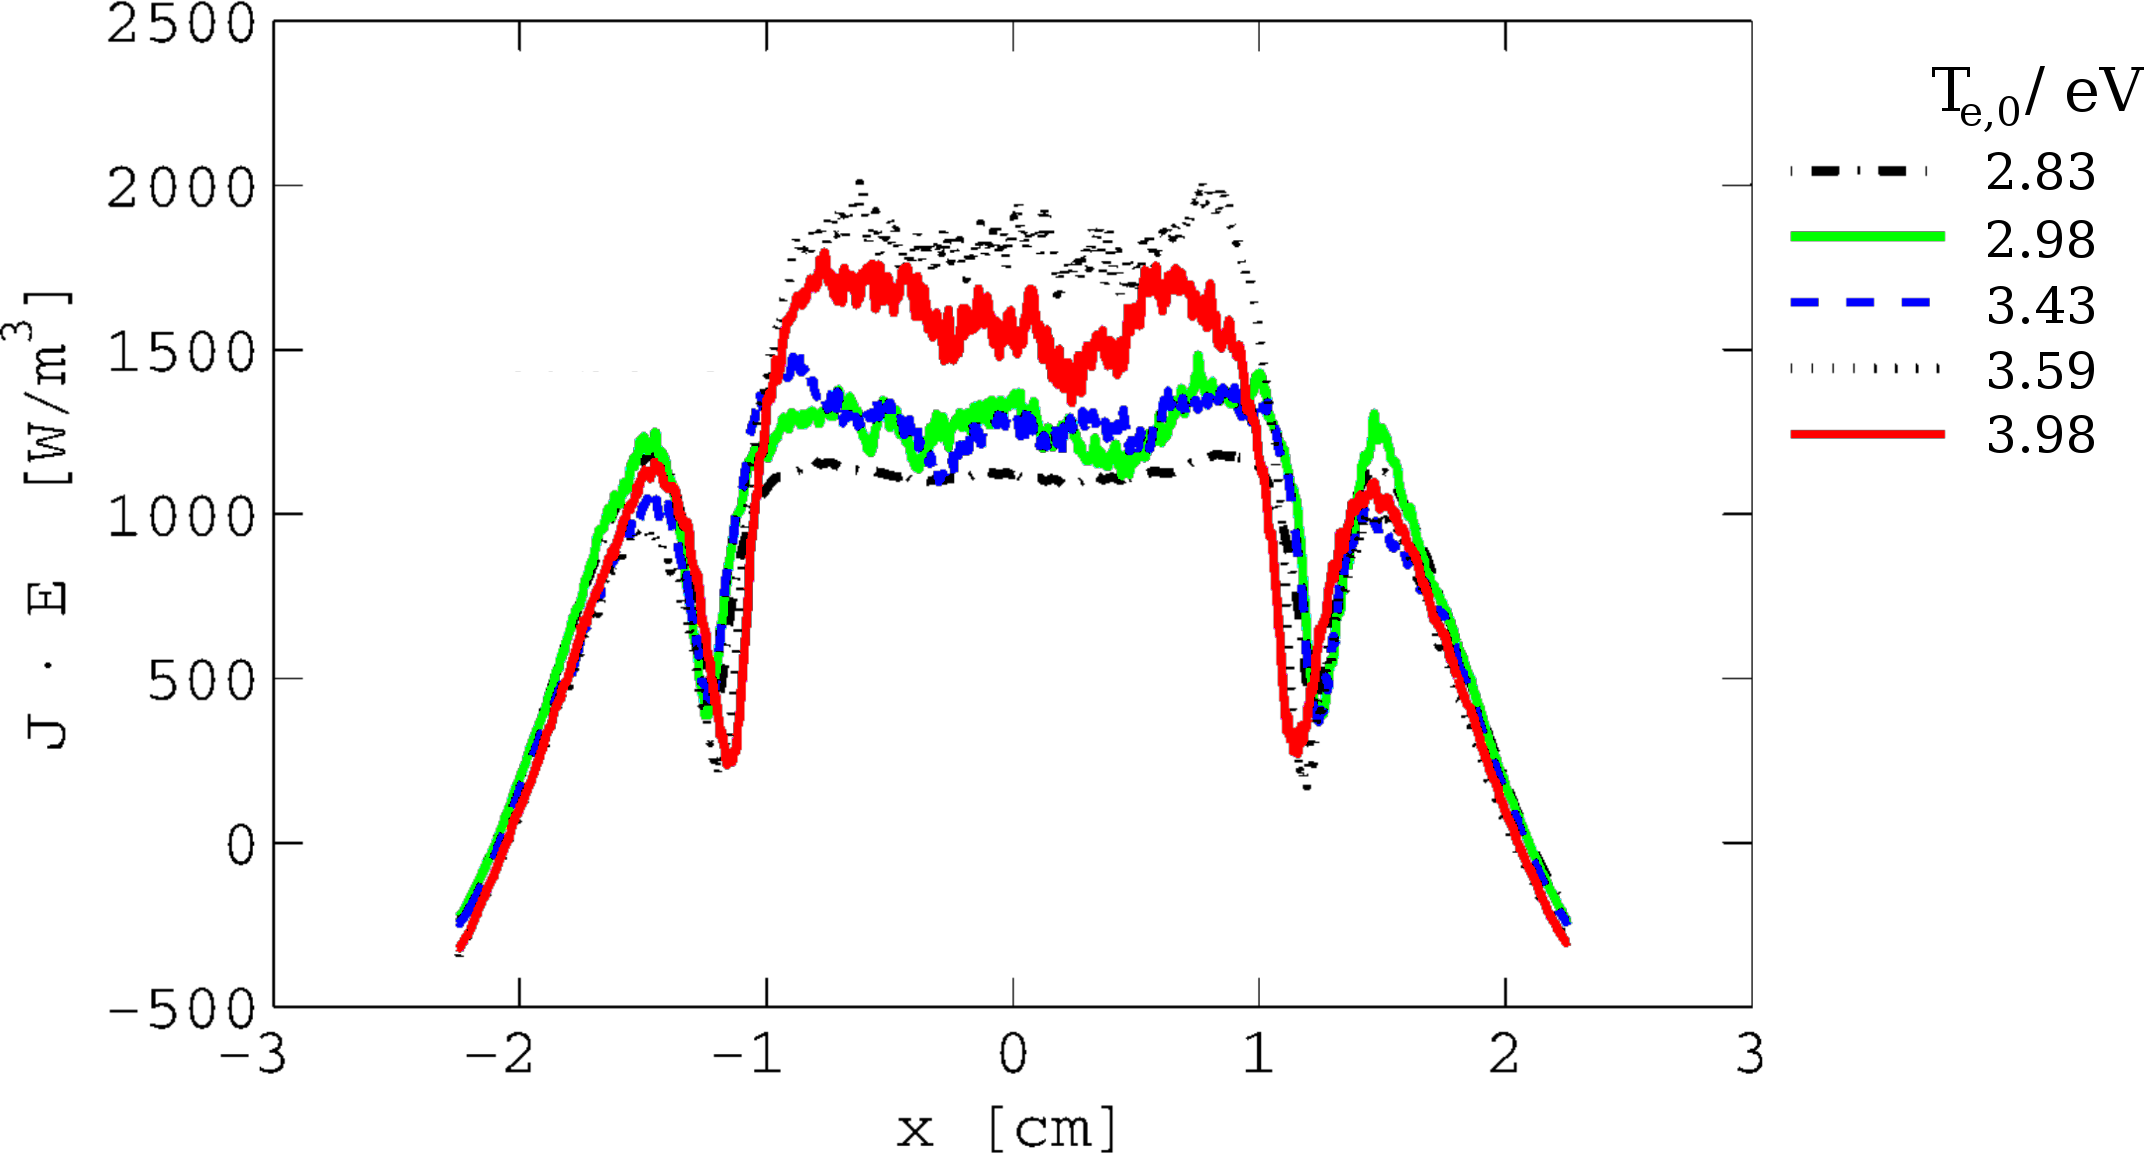
\includegraphics[width=0.8\textwidth]{figures/heatingcomparison.png}
			\caption{%
			Electron heating rate for a ccrf discharge of parallel plates at $\SI{6.7}{\pascal}$ with an electrode gap of $\SI{4.5}{\centi\metre}$ at $\unit[222]{V}$.~\cite{Gudmundsson13}}
			\label{fig:heatingcomparison}
		\end{figure}
%
		\begin{align}
			K=\alpha\,\beta\,\frac{U\ix{sb}}{\epsilon E}\,,%
			\quad\Leftrightarrow\quad%
			E\,<\,m\ix{e}\,\omega^{2}s\ix{0}\,l\,\frac{U\ix{rf}}{U\ix{sb}}\,.%
			\label{equ:randomization}
		\end{align}
%
		The parameter $K$ defines the degree of randomisation. It is derived in~\autoref{equ:randomization} as a measure of phase-space chaos by electron movement. Chaotic motion occurs in this mapping for $K>1$~\cite{Goedde88}. It decreases with increasing energy, so the system is less stochastic at higher energies. This is due to the shrinking phase shift across the discharge volume with higher energies. Hence phase correlations between successive collisions in and with the plasma sheath reduce stochasticity.\\
		One can calculate the instantaneous power dissipated into the plasma due to this heating mechanism. Here, using the sheath speed $u\ix{s}$ from above, the electron drift velocity $u\ix{e}$ and the Maxwell electron velocity distribution function $f\ix{v}(v\ix{e},t)$, Lieberman~\cite{Lieberman88} finds
%
		\begin{align}
			P\ix{stoc}(t)=-2m\ix{e}\int_{u\ix{s}}^{\inf}\,u\ix{s}%
			{\left(v\ix{e}-u\ix{s}\right)}^{2}\,f\ix{v}(v\ix{e},t)\diff v=%
			2\,n\ix{e,0}u\ix{e}k\ix{B}T\ix{e}\sin(\omega t)\,.%
			\label{equ:powerdepositheat}
		\end{align}
%        
%        The change in velocity in one pass through the sheath becomes the impulse approximation of the \emph{Fermi acceleration}m which is written as:
%
%		\begin{align}
%			\Delta v=v\ix{n+1}-v\ix{n}=-2\,\omega\,%
%			s\ix{0}\frac{U\ix{rf}}{U\ix{sb}}\,\sin\varphi\ix{n}\,.%
%			\label{equ:deltavheating}
%		\end{align}
%	
%
%		The results on the right-hand-side yields not net heating if averaged over one rf cycle, if the current used would be conserved in a manner the HWA is predicting it, or the electron drift velocity does not satisfy the Maxwellian distribution function. Hence there have to be deviations from the proposed theory of stochastical heating. This would be e.g.\@ ab initio information about the EEDF, unconsidered transit time effects of the sheath electric field and neglected particle losses and current conservation.\\
%		There are more theoretical approaches on the heating in low-pressure, low-temperature rf plasma. For example, Surendra et al~\cite{Surendra93} put forth the idea that the compression and decompression of the electron density volume between opposing plasma sheaths generates heat inside the bulk, which is responsible for the observed heating.\\
%		The electron heating profile is shown in~\autoref{fig:heatingcomparison}, with peaks near the sheath edges due to stochastic heating while the main plateau in the bulk is a result of the dominantly strong ohmic heating with slow electrons and neutral gas friction.
%		
%		!!!IN WELCHEM REGIME SIND DEINE SIMULATIONEN? IST DIESE DETAILDISKUSSION DAHER WIRKLICH NÖTIG?!!!		Consider the sheaths electric field as constant, $E=U\ix{sb}/s\ix{0}$, the bulks expansion to be $l$ and the sheaths thickness $d$ being modulated cosinusoidal. The equation of motion for an electron in the sheath is taken from above, cancelling out the part of ohmic neutral gas heating.
%
%		\begin{align}
%			d(t)\approx s\ix{0}\left(1+\frac{U\ix{rf}}{U\ix{sb}}\cos\left(\omega t\right)\right)%
%			\label{equ:sheaththickness}
%		\end{align}
%
%	    The \autoref{equ:heatingmotion} is introduced to be dimensionless with the substitution of the corresponding parameters: $\alpha=m\ix{e}\omega^{2}s\ix{0}^{2}/(eU\ix{sb})$, $\beta=U\ix{rf}/U\ix{sb}$ and $\epsilon=s\ix{0}/l\,$. Integration yields the velocity $\mu(\tau)$ of an electron as it moves through the sheath. The transit time $\tau$ is considered for one pass through the sheath of the particle. It can be used to calculate the change in velocity experienced by the electron on each bounce between this oscillating and a fixed wall --- this would be the lowest order \emph{fermi acceleration}. Assuming there are two distinct moments and positions, where the particle enters (index $n$) and re-enters (index $n+1$) the sheath, this gives, using $\varphi\ix{n}$ the phase of the sheath, for the transit time and velocity~\cite{Goedde88}
%		
%		\begin{figure}[t!]
%			\centering
%  		\begin{longtable}{lccccr}
%				\toprule%
%					Case & $\Phi\ix{0}$ & $n\ix{e,0}$/$\unit{m^{-3}}$ %
%					& $n\ix{i-,0}$/$\unit{m^{-3}}$ & $n\ix{i+,0}$/$\unit{m^{-3}}$ %
%					&	$T\ix{e,0}$/$\unit{eV}$ \\%
%		    \toprule\midrule\endhead%
%				1 & 101.30 & \SI{2.43e14} & \SI{1.17e16} & \SI{1.20e16} & 2.83 \\ \midrule%
%				2 & 101.25 & \SI{2.29e14} & \SI{1.21e16} & \SI{1.23e16} & 2.98 \\ \midrule%
%				3 & 101.75 & \SI{2.18e14} & \SI{1.19e16} & \SI{1.20e16} & 2.98 \\ \midrule%
%				4 & 103.11 & \SI{1.55e14} & \SI{1.75e16} & \SI{1.78e16} & 3.59 \\ \midrule%
%				5 & 102.55 & \SI{1.65e14} & \SI{1.70e16} & \SI{1.71e16} & 3.43 \\ \midrule%
%    	\bottomrule%
%			\caption{%
%				Selected plasma parameters for the used cases in~\autoref{fig:heatingcomparison} %
%				at the center of the discharge.~\cite{Gudmundsson13}}\label{tab:comparisonheating}
%			\end{longtable}
%		\end{figure}
	%
	\section{Oxygen Plasma Chemistry}\label{sec:negionphysics}
%
		In comparison to most inert working gases in ccrf discharges, oxygen has an overwhelming number of reaction sets for collisions of elastic, inelastic and reactive character. Additionally, the negative ion species has to be taken into account when discussing collisional processes. For example, an in-depth benchmarking of both simulated and experimentally measured cross section data is given by Gudmundsson et al.\@ in~\cite{Gudmundsson13}. There, 33 collisions and reactions have been revisited, already reducing the investigation to the most important processes in ccrf plasma. In this thesis the selection of possible reactions will be based on~\cite{Bronold07b} and slightly modified. The final collection of cross sections can be found in~\autoref{tab:cross_sections} and observed in~\autoref{fig:cross_sections}. Those data are semi-empirical, meaning part of them are based on measurements in finite energy ranges and low-/high-energy asymptotic models. Cross sections for very high energies are not important, as the collision probability usually decays very fast here.\\
		As already seen in~\autoref{sec:heating}, collisions strongly influence the particle distribution functions and density profiles. Furthermore, a good understanding of the plasma chemistry is key to, e.g.\@ applications in surface physics supported by gas discharges. Of high importance for plasma-assisted material processes is the generation of negative ions. Hence the ratio $\alpha=n\ix{i,-}/n\ix{e}$ is important to characterize the electronegative plasma, like a ccrf oxygen discharge by $\alpha>1$.\\
		I will highlight the most important collisions and reactions in the following section. 
%
		\begin{longtable}{lll}
			\toprule%
				\bfseries Nr. & \bfseries Reaction & \bfseries Type \\%
			\toprule\midrule\endhead%
						& \bfseries Elastic scattering 							& \bfseries Energy loss 	\\% 
						$(1)$  & $e^{-}+O\ix{2}			 	\rightarrow	O\ix{2}+e^{-}$ &						\\%
						$(2)$  & $O^{-}+O\ix{2}			 	\rightarrow	O\ix{2}+O^{-}$ & 						\\%
						$(3)$  & $O\ix{2}^{-}+O\ix{2} \rightarrow	O\ix{2}+O\ix{2}^{-}$ & 			\\ \midrule%
						& \bfseries Electron energy loss scattering & \bfseries Energy loss 	\\%
						$(4)$  & $e^{-}+O\ix{2}			 	\rightarrow	O\ix{2}^{\nu}+e^{-}$ & %
										Vibrational excitation	($\nu=1,\dots,4$)											\\%
						$(5)$  & $e^{-}+O\ix{2}			 	\rightarrow	O\ix{2}(Ryd)+e^{-}$ & %
										Rydberg excitation																						\\%
						$(6)$  & $e^{-}+O\ix{2}			 	\rightarrow	O(1D)+O(3P)+e^{-}$ & %
										Dissociative excitation at $\SI{8.6}{\electronvolt}$					\\%
						$(7)$  & $e^{-}+O\ix{2}		 	 	\rightarrow	O\ix{2}%
																					 (a^{1}\Delta\ix{g},b^{1}\Sigma\ix{g})$ & %
										Meta-stable excitaion																					\\ \midrule%
						& \bfseries Electron and ion reactions & \bfseries Creation and loss 	\\%
						$(8)$  & $e^{-}+O\ix{2}^{+}	 	\rightarrow	2\,O$ & %
										Dissociative recombination 																		\\%
						$(9)$  & $O^{-}+O\ix{2}^{+}	 	\rightarrow	O\ix{2}+O$ & %
										Neutralization						 																		\\%
						$(10)$ & $e^{-}+O\ix{2}	 		 	\rightarrow	O+O^{-}$ & %
										Dissociative attachment		 																		\\%
						$(11)$ & $O^{-}+O\ix{2}			 	\rightarrow	O+O\ix{2}+e$ & %
										Direct detachment 																						\\%
						$(12)$ & $e^{-}+O\ix{2}		 		\rightarrow	2e^{-}+O\ix{2}^{+}$ & %
										Impact ionization 																						\\%
						$(13)$ & $e^{-}+O^{-}			 		\rightarrow	O+2e^{-}$ & %
										Impact detachment																							\\%
			\midrule\bottomrule%
			\caption{%
				Most important collision and reactions in ccrf plasmas. %
				Empirical and simulated data, which have been included in %
				this simulation are shown in~\autoref{fig:cross_sections}.}\label{tab:cross_sections}	
		\end{longtable}	

	%		
		\subsection{Collisions and Reactions}\label{sec:negiondynamics}
%	
			\paragraph{Elastic Scattering}%
			The elastic collisions of $(1)$--$(3)$ conserve the particle numbers. Those are inter-species scattering processes, which will be assumed to have an isotropic inincident angle dependency~\cite{Bronold07b}. Intra-species elastic collisions were not very important at the selected parameter regions, though ion-ion scattering can strongly incluence the IEDF structure of the concerned densities are very high. However, for the electron species a binary \emph{coulomb scattering} process was used: the scattering angle $\chi$ is given by~\autoref{equ:coulomb_scatter} with $v\ix{rel}$ the relative velocity, $\ln\Gamma$ the Coulomb logarithm (see~\autoref{tabe:physicalquantities}) and $\tau\ix{c}$ the collision time.
%
			\begin{align}
				\langle\tan^{2}\frac{\chi}{2}\rangle=\frac{e^{4}n\ix{e}\ln\Gamma}%
					{8\pi\varepsilon\ix{0}m\ix{e}^{2}v\ix{rel}^{3}}\tau\ix{c}%
				\label{equ:coulomb_scatter}	
			\end{align}	
%
			The~\autoref{fig:cross_sections} shows the corresponding cross sections. In fact, only two are elastic processes, where as the collision of $O\ix{2}^{+}$ and the neutral molecule is a charge exchange reaction with momentum transfer. This kind of process:
%
			\begin{align}
				A^{-/+}+B\rightarrow A+B^{+/-}%
				\label{equ:charge_exchange}
			\end{align}
%
			is important for the consideration of surface effects. An ion with greater than thermal velocity coming from the wall will be cooled down by charge exchange collisions, which will transfer heat into the neutral reservoir.
%			
			\paragraph{Electron Energy Loss}
			Electron energy loss occurs due to inelastic collisions $(4)$--$(7)$, where an oxygen molecule is excited or dissociated into fragments. Here, the spatio-temporal evolution of the molecule or the fragments are of no interest for this thesis. Hence they are treated as `test collisions', in which only the electrons lose momentum and change direction. Again, the neutral particle reservoir is considered to equilibrate at a sufficiently short time scale $<\unit[\tenpo{-15}]{s}\,$. Rotational excitations are found to be unimportant, though the vibrational parts considerably influence the EEDF~\cite{Gudmundsson13}. The isotropic post-collision relative velocity change in the center-of-mass system gives
%
			\begin{align}
				\widetilde{v}\ix{rel}=\sqrt{v\ix{rel}^{2}-\frac{2\Delta E}{\mu\ix{i,j}}}\,.%
				\label{equ:electron_energyloss}
			\end{align}
%
			The most important electron energy loss scattering is the vibrational and electronic excitation, as well as the dissociation of the oxygen molecule.
%
			\paragraph{Electron and Ion Channels}
			The last class of collisions concerned here are the electron and ion production processes. Collisions $(8)$ and $(9)$ are the annihilation of the two oppositely charge particles. Those are namely recombination processes. The ion-ion neutralization is constructed by a \emph{Landau-Zener} model, where the adiabatic energy of the ($O^{-}$,$O\ix{2}^{+}$) configuration decreases when the particles approach each other. At the critical distance $R\ix{c}$ this energy drops bellow the one of the ($O$,$O\ix{2}$) configuration, yielding the probability to change states $\sigma\ix{r}(E)$ 
%
			\begin{align}
				\sigma\ix{r}(E)=4\pi R\ix{c}^{2}\left(1+\frac{1}{R\ix{c}E}\right)\,.%
				\label{equ:neutralization}
			\end{align}
%			
			The dissociative attachment $(10)$ and direct detachment $(11)$ are treated as binary collisions, like the elastic electron scatter process. For the dissociative attachment from the ground state oxygen molecule a threshold energy of $\SI{4.2}{\electronvolt}$ is needed. The incident electron loses this energy to the $O\ix{2}^{-}$, which afterwards breaks up into the two fragments. The electron transition time is, again, assumed to be short on a nuclear timescale and the resulting particles share the remaining kinetic energy of the incident electron.\\
			In the experiment there is a second stage for the direct detachment process: through associative detachment, oxygen atom, electron and molecule form an ozone $O\ix{3}$ particle. This most likely due to the presence of meta-stable $O\ix{2}(a^{1}\Delta\ix{g})$. After the necessary threshold energy of $\SI{1.3}{\electronvolt}$ has been supplied to directly detach $O^{-}$ on an oxygen molecule, the afore-mentioned detachment takes no energy whatsoever, making it a potentially important loss channel for cold $O^{-}$ ions.\\
			For impact ionization $(12)$ and detachment $(13)$ the following is assumed: first, an inelastic binary collision takes place, in which the electron loses the necessary reaction energy. The post-collision oxygen particle is afterwards split into an additional $e^{-}$ and atom/ion ($O^{-}$/$O$), which proceed to perform an elastic binary collision. During this process, energy and momentum conservation is satisfied, ensuring numerical stability.\\

%			
			\begin{figure}[!b]
				\centering
				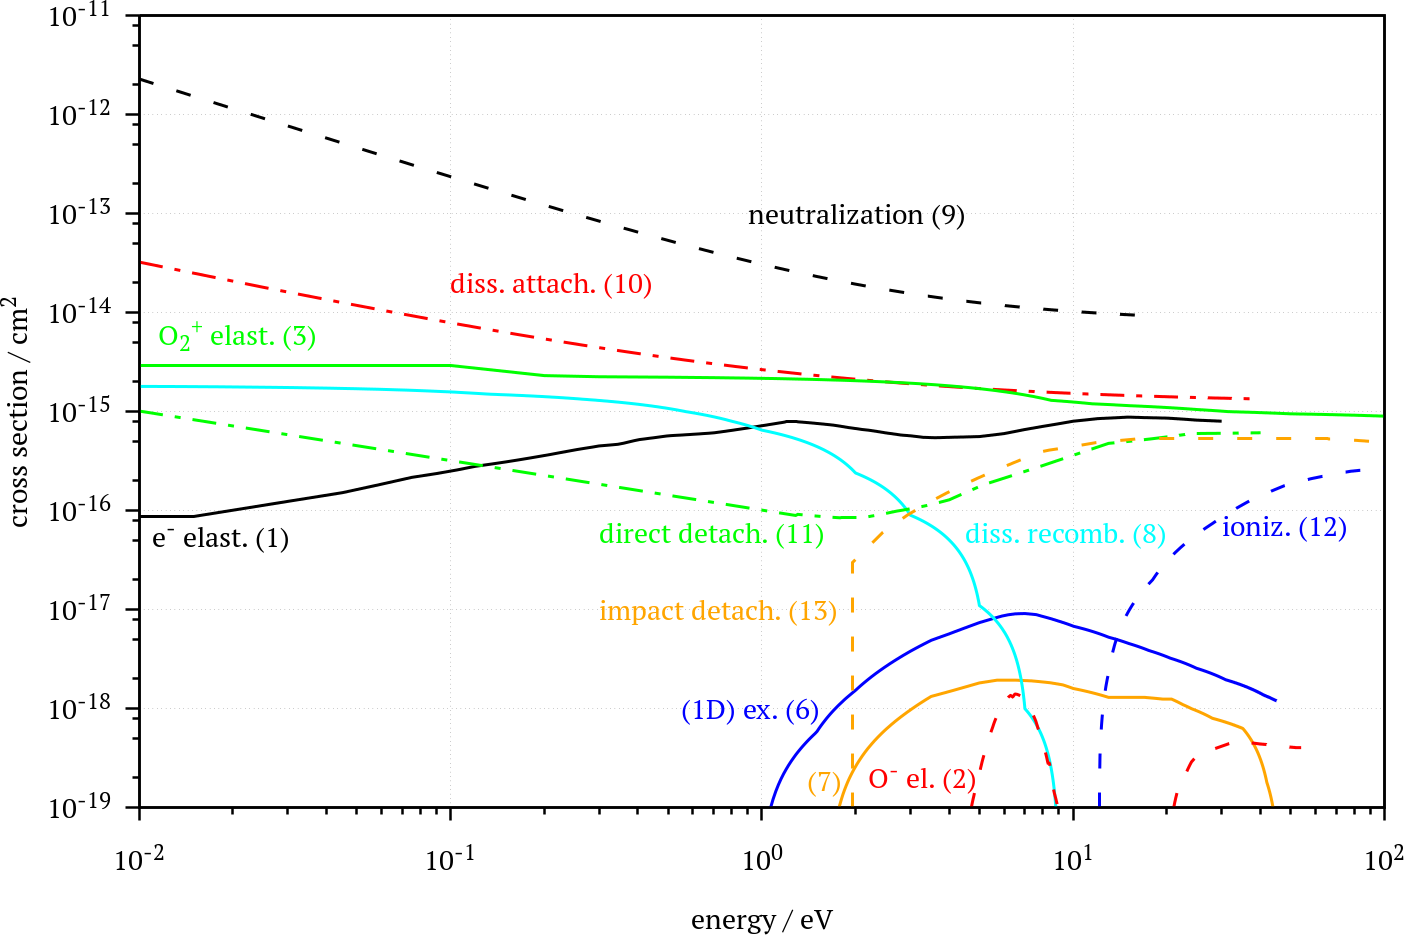
\includegraphics[width=1.0\textwidth]{figures/xsections.png}
				\caption{%
				Cross section data of electron energy loss, electron and ion production/loss and elastic scattering collisions from~\cite{Gudmundsson13} and~\cite{Bronold07b}. The corresponding reaction equations are shown in~\autoref{tab:cross_sections}.}%
				\label{fig:cross_sections}	
			\end{figure}	

	%			
		\subsection{Anion Species}\label{sec:anionproduction}
%
			The main production channel of negative oxygen ions in ccrf disharges at low pressures and temperatures is the dissociative attachment reaction $(10)$. Here, an electron becomes attached to a molecule. The successive electronic excitation is of short duration and does not change the intra-molecular distance. Afterwards, there is a significant chance of transition to a dissociative state exists, which has a lower equilibrium energy at greater intra-nuclear distances. Hence, the dissociation of this molecule is rather likely.
%
			\begin{align}
				e^{-}+AB\rightarrow A+B^{-}%
				\label{equ:dissociative_attach}
			\end{align}
%
			Another possible creation channel is a three-body collision of non-dissociative character, whose cross sections is magnitudes smaller than the one of \autoref{equ:dissociative_attach}. Hence I will only consider dissociative attachment reactions $(10)$ for the anion production.\\
			Negative ion loss can happen through reactions $(11)$, $(13)$ and $(9)$. The latter is the only collision with a cross section larger than the creation via dissociative attachment (see~\autoref{fig:cross_sections}). For all relative energies, the neutralization has a probability of at least one magnitude larger than the other channels. Cross sections of direct $(11)$ and impact $(13)$ detachment are, depending on the energy, about one to two orders of scale smaller.\\
			In general, the produced negative ions are cold. The anion distribution reaches until the boundaries of the bulk, where processes with large cross sections at low energies become important~\cite{Bronold07b}. Those reactions would be ion-ion neutralization and associative detachment. Direct detachment, though being still present around $E<\unit[1]{eV}$, has an energy threshold and is not significant for this region. Furthermore, the probability of neutralization $(9)$ is proportional to the $O\ix{2}^{+}$-density. Bronold et al.\@ proposes, that the production and loss of $O^{-}$ is rather insensitive to voltage changes up to $\unit[300]{V}$. Furthermore, the most important range for incident energies will be $4$--$\unit[15]{eV}$, while the EEDF is rather voltage-independent.\\
			Considering the physics of a negative ion --- $O^{-}$ follows the same dynamic and kinetic behaviour as the electrons, but is easily confined by the plasma potential due to their much greater mass and, hence $\omega\ix{p,i-}<<\omega\ix{p,e}$ --- the main loss and production channels are most prominent in the bulk. Therefore, a low-pressure, low-temperature ccrf discharge has an electronegative core, in which the cold anions are captured, and areas where they are excluded. The presence of negative ions also has a great impact on the distribution functions of other plasma species. It is possible to form a quasi-neutral volume core, consisting only of ion species, and a peripheral electron-ion plasma in the discharge sheaths. At pressures $>\unit[30]{Pa}$ and large input powers, the value of electronegativity $\alpha$ leads to instabilities between ionization and electron attachment reactions. The electron density peaks, where as the corresponding temperatures drops. Because of the strong negative ion coupling, the $O^{-}$ density fluctuates as well.

	%
    \newpage
	\section[Particle-in-Cell Simulations with Monte Carlo-Collisions]%
	        {Particle-in-Cell Simulations with \\Monte-Carlo-Collisions}\label{sec:picsimulationmcc}
%
	Particle-In-Cell simulations with Monte-Carlo-Collisions (PIC-MCC) represent a powerful tool for fully kinetic plasma studies, with inclusion of complicated reaction/collision routines, as well as field solving methods. Hence they are used in all branches of plasma physics, ranging from simple labaratory discharges to electric propulsion devices and interplanetary astrophysical system. This kind of computer code simulates the motion of pseudo-particles in a continuous 1d3v-/2d3v phase-space. Macro-quantities like forces, fields and densities are stored and calculated on a mesh with constant intervals. The computational cost sums up to $N\log(N)$ per timestep --- with $N$ the total particle number --- because the self-consistent electrostatic macro-fields are calculated by solving \emph{Poisson's equation}, and no particle-particle interactions are considered.\\
	In the following section the motivation and basic scheme of a PIC-MCC simulation will be highlighted. Accordingly, the collision routines will be layed out, as well as the transition from a 1d3v to a 2d3v model. As it was mentioned in~\autoref{sec:chapter_ccrfbasics}, I will focus on the electrostatic case with $\vec{B}=0$, as the magnetic field generated from the moving charged particles is small enough that the force of $q\ix{j}(\vec{v}\ix{j}\times \vec{B})$ is negligible in comparison to $q\ix{j}\vec{E}$. 
%	
		\subsection{Principles}\label{sec:picbasics}
%
		In general, the spatio-temporal evolution of the velocity distribution function $f\ix{j}(\vec{v},\vec{r},t)$ is given by the \emph{Boltzmann equation}:
%
			\begin{align}
				\frac{\partial f\ix{j}}{\partial t}+\vec{v}\cdot\nabla_{\vec{r}}\,f\ix{j}%
					+\frac{q\ix{j}}{m\ix{j}}\vec{E}\cdot\nabla_{\vec{v}}\,f\ix{j}%
					=\left(\frac{\partial f\ix{j}}{\partial t}\right)\ix{Coll}\,.%
				\label{equ:boltzmannequation}
			\end{align}
%
			In this equation, the product of $q\ix{j}\vec{E}/m\ix{j}$ denotes the electrostatic force onto the particle of species $j$. The velocity and space gradient are calculated like $\nabla_{\vec{r}}\,f\ix{j}=\partial f\ix{j}/\partial x\cdot\vec{e}\ix{x}+\dots$ and so on. The right hand side of $(\partial f\ix{j}/\partial t)\ix{Coll}$ is the sum of all collision effects on $f\ix{j}(\vec{v},\vec{r},t)$. An approach would be an integral form, in which all probabilities of a two-body interactions with different incident and outgoing velocities are summed up in a convolution integral with $f\ix{j}(\vec{v},\vec{r},t)$.\\
			The approach via the distribution function yields the advantage of an easy access to the afore-mentioned macro-quantities, the zeroth and first moment are noted below in~\autoref{equ:zeorthandfirstmoment}. Using the moments, one can write down $f\ix{j}(\vec{v},\vec{r},t)$ at a thermodynamic equilibrium of $T\ix{j,0}$ as the \emph{Maxwell-Boltzmann-distribution-function} in~\autoref{equ:maxwellboltzmannfunction}.
%
			\begin{align}
				n\ix{j}(\vec{r},t)=q\ix{j}\int_{-\infty}^{\infty}%
					f\ix{j}(\vec{v},\vec{r},t)\diff\vec{v}\,,%
					\quad\quad%
					\langle v\ix{j}(\vec{r},t)\rangle=\frac{1}{n\ix{j}(\vec{r},t)}%
					\int_{-\infty}^{\infty}\vec{v}f\ix{j}(\vec{v},\vec{r},t)\diff\vec{v}%
				\label{equ:zeorthandfirstmoment}\\[0.3cm]
				f\ix{j}(\vec{v},\vec{r},t)=\frac{n\ix{j}(\vec{r},t)}{q\ix{j}}\,\hat{f}\ix{j}(\vec{v},\vec{r},t)%
					=\frac{n\ix{j}(\vec{r},t)}{q\ix{j}}\,{\left(\frac{m\ix{j}}{2\pi k\ix{B}T\ix{j,0}}\right)}^{3/2}%
					\,\exp\left(-\frac{|\vec{v}\ix{j}|^{2}}{v\ix{j,th}^{2}}\right)%
				\label{equ:maxwellboltzmannfunction}
			\end{align}
%
			In a Maxwellian plasma one could use a fluid dynamic approach, where the equations of motion for a single particle are multiplied with the number density function. This would reduce the computational cost drastically, as one would no longer have to track each particle individually, and sufficiently describe the discharge by charaterization of macro-quantities. This is true, if mean-free-paths are small and collisions rather likely, hence the afore-mentioned distribution function correct. In a low-temperature, low-pressure ccrf discharge mean-free-paths are large and collisions are rare, which is why a fully kinetic Particle-in-Cell simulation method is used.\\
			Satisfying the above requirements, the $n$-th equation of motion in the $N$-particle system becomes:
%
			\begin{align}
				\frac{\diff \vec{x}\ix{n}}{\diff t}=\vec{v}\ix{n}\,,%
					\quad\quad\quad%
					\frac{\diff \vec{v}\ix{n}}{\diff t}=\frac{1}{m\ix{n}}%
					\vec{F}\ix{n,L}(\vec{x}\ix{n},\vec{E},t)%
					=\frac{q\ix{n}}{m\ix{n}}\vec{E}(\vec{x}\ix{n},t)%
				\label{equ:equationofmontionpic}
			\end{align}
%
			where $F\ix{n,L}$ is the \emph{electrostatic Lorentz force}.\\
			First, the global charge density is calculted by interpolating the point charges $q\ix{n}$ of each particle onto the afore-mentioned fixed mesh grid (~\autoref{equ:interpolation}~). Next, the Poisson's equation is solved globally on that grid (~\autoref{equ:poissonpotential}~), using the interpolated density. At last, the Maxwell'is~\autoref{equ:efieldmaxwell} yields the electric field.
%
			\begin{align}
				\rho(\vec{r},t)&=\rho(\vec{x}\ix{1},\vec{x}\ix{2},\dots,\vec{x}\ix{N},t)%
					\label{equ:interpolation}\\[0.0cm]
				\Rightarrow%
				\Delta\Phi(\vec{r},t)&=-\frac{\rho(\vec{r},t)}{\varepsilon\ix{0}}%
					\label{equ:poissonpotential}\\[0.0cm]%
					\Rightarrow\hspace*{7pt}%
				\vec{E}(\vec{r},t)&=-\nabla\Phi(\vec{r},t)%
					\label{equ:efieldmaxwell}
			\end{align}
%
			The number of $N$ is of orders of magnitude higher than what the best supercomputers can handle. Hence it is assumed that one simulated particle at $\vec{x}\ix{n}$ and veloctiy $\vec{v}\ix{n}$ represents many physical particles. This \emph{superparticle factor} is usually between $\tenpo{3}$--$\tenpo{4}$, depending on the size and initial density in the simulated domain. Those superparticles follow the same dynamic and kinetic behaviour like their physical counterparts, assuming that all other relevant parameters are scaled accordingly.\\
			Furthermore, the time is also divided into discrete partitions, which yields the simulation time for a constant stept width $\Delta t$: $t\rightarrow t\ix{k}=t\ix{0}+k\, \Delta t$ (and correspondingly all other physical properties). Here, a \emph{leap frog} scheme (`Boris pusher') is used to calculate the velocities, in contrast to other time-dependent attributes, which still has a sufficient accuracy, stability and short computational time. With each calculation step, the error scales with $\sim\Delta t^{2}$ and fulfills the requirement for numerical stability $\Delta t^{\alpha>1}$. The explicit leap frog solution is calculated with old quantities of the previous timestep, thus it is simpler and faster. The single drawback on this method would be the requirement of a smaller timestep, e.g\@ $\Delta t/2$.\\
			The most significant part of the simulation code is the \emph{particle mover} or \emph{particle pusher}, in which the new positions and velocities calculated. For each particle of index $n$ and species $j$ the following equations have to be solved at a given time step $k$, or $k+/-\frac{1}{2}$ respectively:
%
			\begin{align}
				\vec{u}\ix{n,+}=\vec{v}\ix{n,k-1/2}+h\cdot\vec{E}\ix{k}\,,%
					\quad\quad%
					h=\frac{q\ix{j}}{2\,m\ix{j}}%
					\nonumber
				\end{align}\vspace*{-0.8cm}\begin{align}
				\boxed{%
					\vec{x}\ix{n,k+1}=\vec{x}\ix{n,k}+\Delta t\vec{v}\ix{n,k+1/2}%
						\quad\text{~and~}\quad%
						\vec{v}\ix{n,k-1/2}=\vec{u}\ix{n,+}+h\cdot\vec{E}\ix{k}%
						\label{equ:leapfrogscheme}%
				}
			\end{align}
%
			The field, potential and density only have to be calculated once per time step. Though this requires less effort, the calculation of $\vec{E}$, $\Phi$ and $\rho$ need to be done in this case by one processing core. The equation~\autoref{equ:interpolation} and following are solved globally. A simple approach to obtain the solution of Poisson's equation is the \emph{finite-difference method}. For a two-dimensional, with $\Delta r$ equally partitioned mesh at ($r^{(1)}\ix{l}$,$r^{(2)}\ix{m}$) one yields the \emph{five point stencil}:
%
		\begin{align}
			4\Phi\ix{l,m}-\Phi\ix{l-1,m}-\Phi\ix{l+1,m}-\Phi\ix{l,m-1}-%
				\Phi\ix{l,m+1}=\Delta r^{2}\cdot\frac{\rho\ix{l,m}}{\varepsilon\ix{0}}%
				\label{equ:fivepointstar}
		\end{align}
%
		While the potential is calculated using~\autoref{equ:fivepointstar}, all but one processing core remain idle and wait for the result to be distributed and used in the particle pusher in~\autoref{equ:leapfrogscheme}.\\
		The universal stability criteria for a kinetic plasma simulation using a PIC method with mesh size $\Delta r$ and time step $\Delta t$ are given by~\autoref{equ:stabilitycriteria}. The spatial and temporal step width should sufficiently resolve the smallest and fastest processes in the simulated model. Hence the physical scales of electron plasma frequency $\omega\ix{p,e}$ and electron Debye length $\lambda\ix{D,e}$ are chosen. The parameters are chosen so that an electron never flies beyond one cell during a single step of time. Also, the interpolation of the macro-quantities yields an error the size of micro-fluctuations between single particles, thus is negligible.
%
		\begin{align}
			\boxed{%
				\Delta t\ix{0} \le \SI{0.2}\cdot\omega\ix{p,e}%
					\quad\text{~and~}\quad%
					\Delta r\ix{0} \le \SI{0.5}\cdot\lambda\ix{D,e}%
					\label{equ:stabilitycriteria}%
				}
			\end{align}
%
			To summarize this section, a basic simulation code cycle for one time step of a PIC-MCC method is shown in~\autoref{fig:picscheme}. A more versatile and in-depth approach on PIC simulations can be found in~\cite{Tskhakaya}.
%
			\begin{figure}[!t]
				\centering
				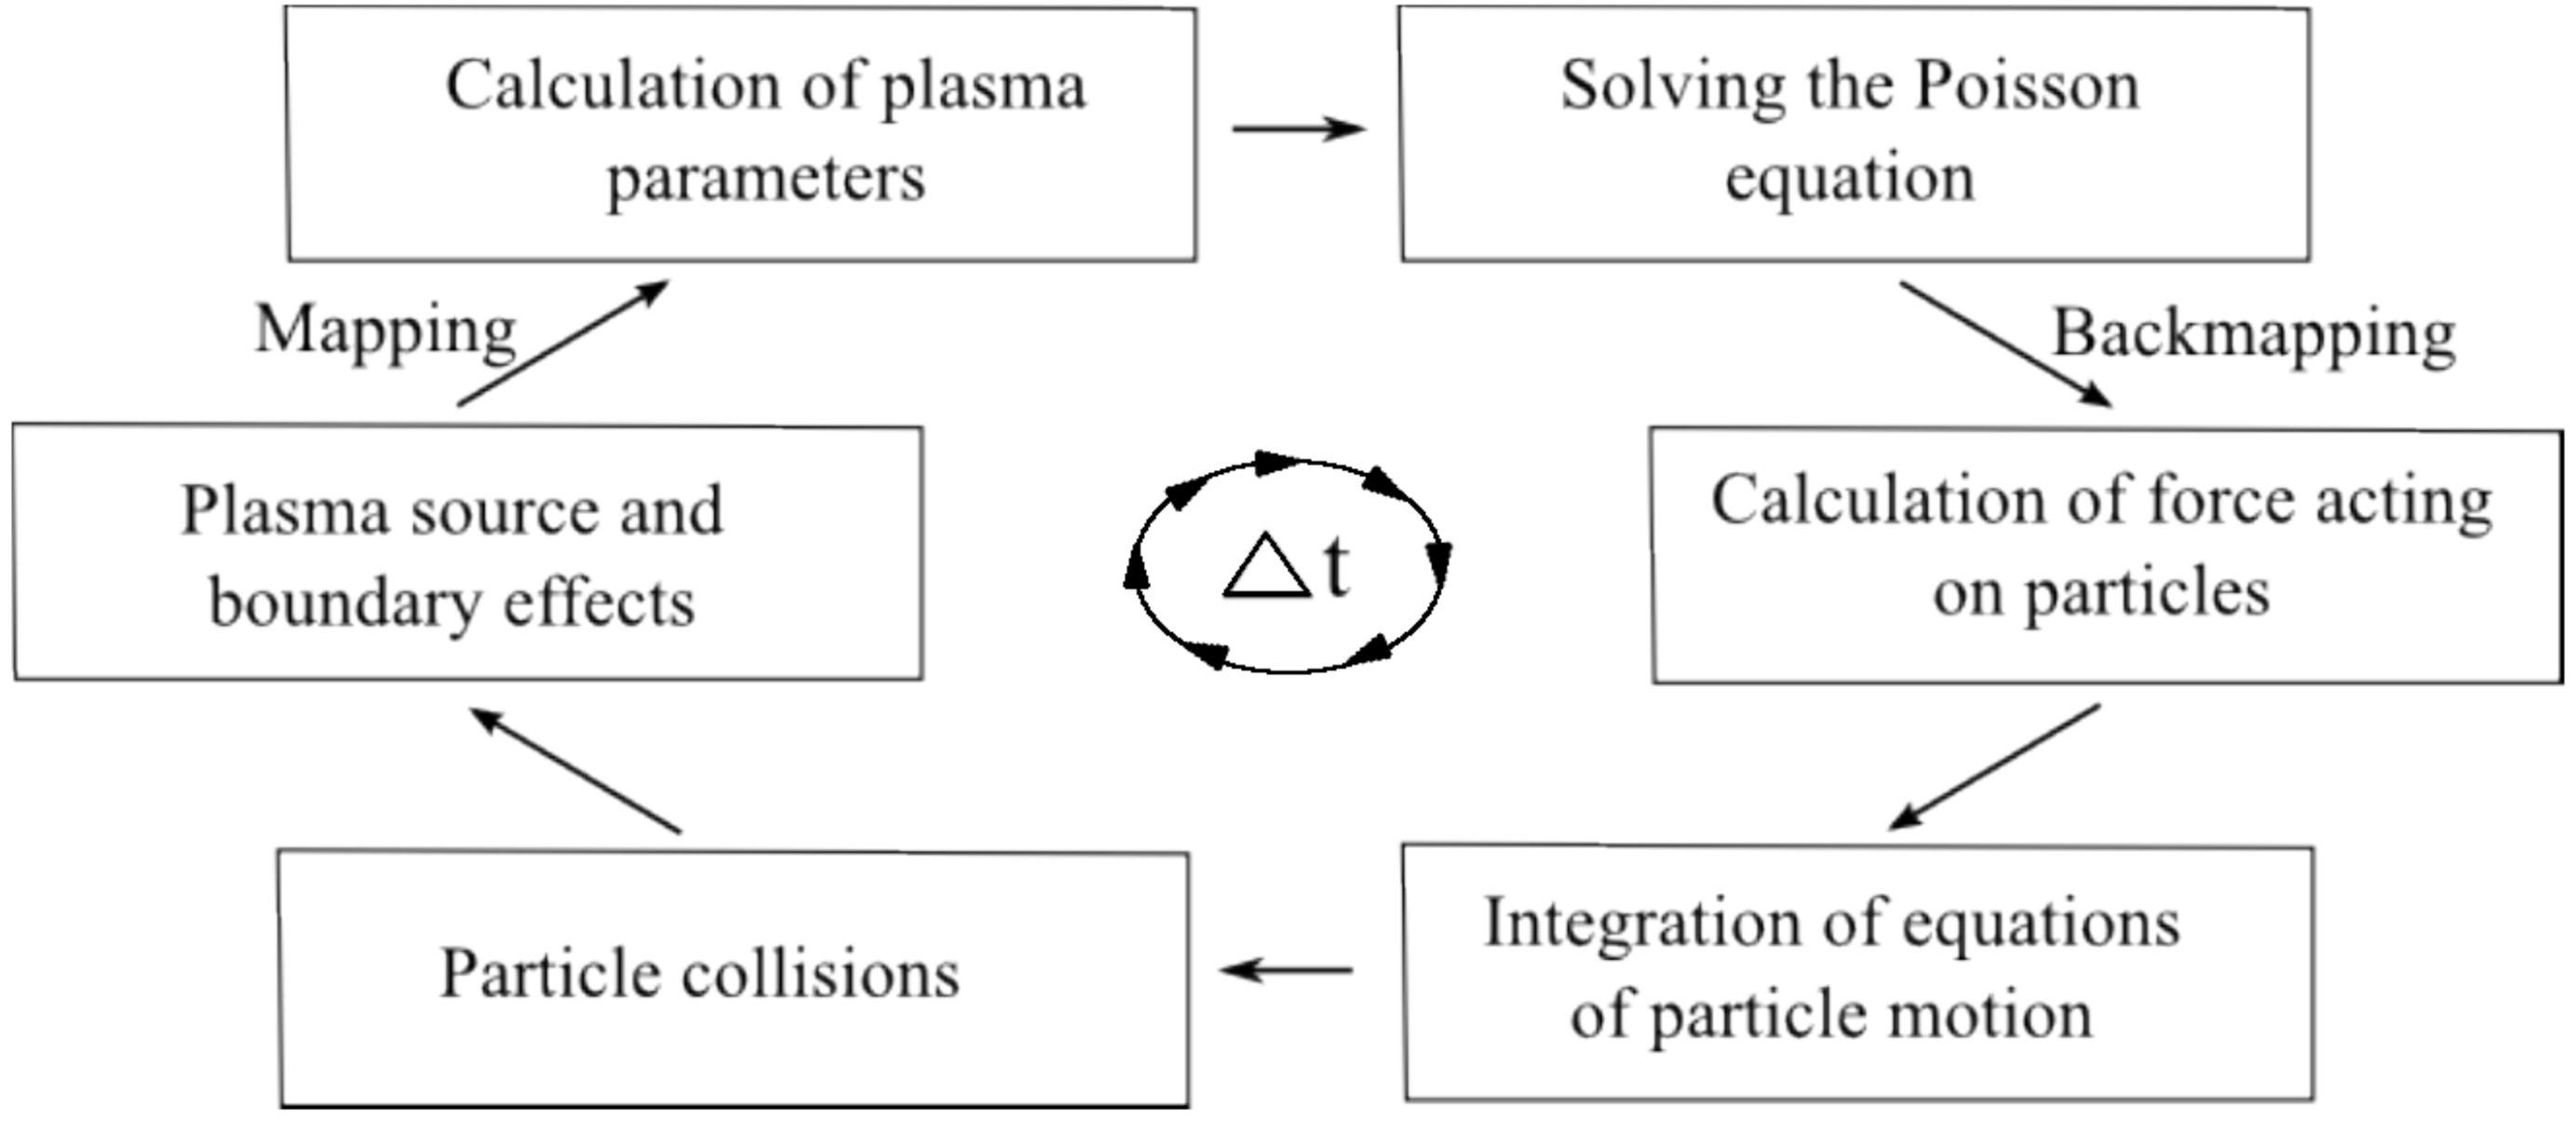
\includegraphics[width=0.8\textwidth]{figures/picscheme.pdf}
				\caption{%
				PIC simulation scheme~\cite{Matthias15}. The code starts with the initilisation of all particle species with their corresponding velocities and a first mapping process, followed by the solution of the Maxwell's equation~\autoref{equ:efieldmaxwell}. Afterwards the main loop with push, collisions, mapping and so on begins.}\label{fig:picscheme}
			\end{figure}

	%
		\subsection{2d3v PIC}\label{sec:pic_2d3v}
%
			In the following, I will highlight the difficult tasks of a spatially twodimensional PIC simulation, refering to the scheme in~\autoref{fig:picscheme}.
%
			\paragraph{Simulation Model}%
			In the beginning of the simulation, before the first calculation step is done, the domain has to be constructed. The cylindrical setup is reduced to the radial and axial dimensions, e.g\@ $(r,z)$ for reasons of symmetry. The five-dimensional phase-space is completed with the full velocity triplet $\vec{v}=(v\ix{r},v\ix{z},v_{\vartheta})$. The two-dimensional mesh expands in radial and axial direction by $N\ix{r}$ and $N\ix{z}$ equally sized partitions respectively. Thus, the area of a single mesh cell is $\Delta r\ix{0}^{2}$. The spatial and temporal discretisation $\Delta r\ix{0}$ and $\Delta t\ix{0}$ are chosen to be dimensionless, so calculations inside the code can be performed much more easily and are less likely to have errors.\\
			Additionally, certain physical properties have to be scaled according to the spatial weight of a cell. Because a `quasi-three-dimensional' cell of coordinates $(n\ix{r},n\ix{z})$ grows in volume with increasing radial index (for a more visual approach, take a look at~\autoref{fig:radialcylinder}), a weighting factor needs to be multiplied with properties like densities and pressure.\\
			Next the particle species have to be initialised. Here, one uses pressure and intial density to model a global distribution of electrons, ion and neutral species. The corresponding super particle factor is used to decrease computational time. Though it has been proven that this does not introduce artifacts to the simulations results --- the equation of motion only depends on a charge-to-mass-ratio --- it should not be too high. Collisions may be underrepresented when there are not enough targets, though in reality $\sim\tenpo{4}$ times the amount of particles would be available.\\
			A number of electrons, ions and neutrals is distributed in each cell, using a Maxwell-distribution-function. Inside one mesh cell the particles are spread random and continuously. The same goes for the velocity, which is randomly picked from the specified distribution function. The radial deformation of each cell has to be taken into account here. Therefore more particles have to be initiated in cells the closer they get to the outer limit of the cylindrical domain.
%
			\paragraph{Potential and Field Calculation}
			After the domain is filled the resulting density distribution, potential and electric field have to be calculated. The charges need to be mapped to the grid points to generate a density, which is used to solve Poisson's equation (see~\autoref{equ:fivepointstar}). A linear weighting function is applied for each charge to form the density. The resulting scheme for a particle at $(r,z)$ in one and two dimensions is shown in~\autoref{fig:cicweighting} and~\autoref{equ:cicweighting}. The index tuple $k,j$ denotes the position in the twodimensional mesh, $n\ix{k,j}$ the corresponding density, $(r\ix{k},z\ix{j})$ the position --- this e.g\@ would be $r\ix{k}=\Delta r\ix{0}\cdot k$ and so on --- and $S\ix{k,j}$ the statistical weight, composed of dimensionless charge, super particle and volume factor. The quotient $A\ix{k,j}=\Delta r\ix{0}^{2}$ normalizes the result, so that no error is made when summarizing all four contributions of a single particle to the density.
%
			\begin{figure}
				\centering
				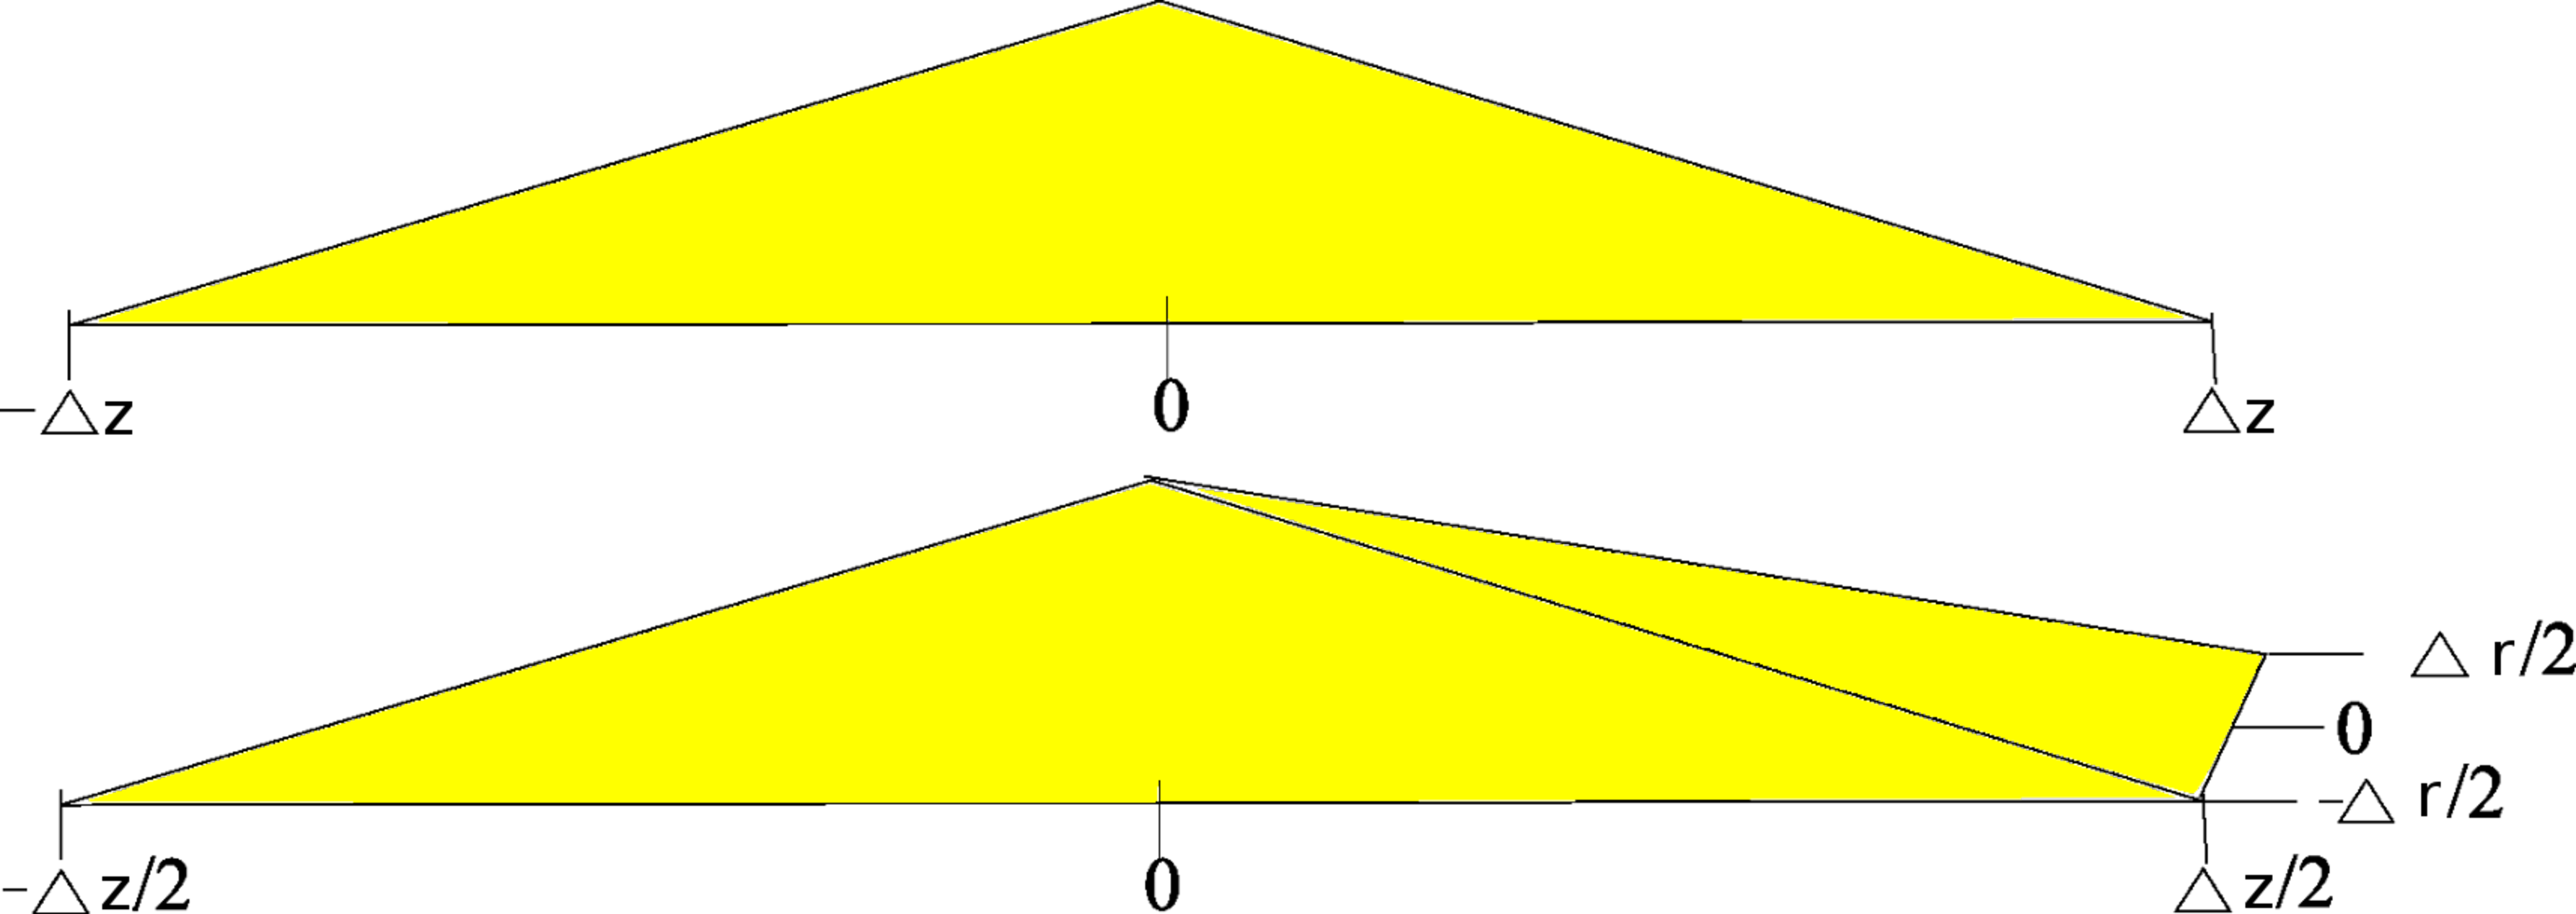
\includegraphics[width=0.8\textwidth]{figures/cicweighting.pdf}
				\caption{%
					Linear weighting scheme for (top) 1D and (bottom) 2D simulations. The latter is an expansion into the radial dimension from a 1D case. The twodimensional approximation is called Cloud-In-Cell (CIC)~\cite{Matthias15}.%
			}\label{fig:cicweighting}
			\end{figure}
%
			\begin{align}
				\text{1D:}\quad\quad\,\,\,\,%
					n\ix{j}&=\frac{S\ix{j}}{\Delta z}\left(z\ix{j}-z\right)%
					\label{equ:cicweighting1d}\\[0.0cm]
				\text{2D:}\quad\quad%
					n\ix{k,j}&=\frac{S\ix{k,j}}{A^{2}\ix{k,j}}%
					\left(r\ix{k+1}-r\right)\cdot\left(z\ix{j+1}-z\right)%
					\label{equ:cicweighting}
			\end{align}
%
			To avoid possible self-forces and satisfy the conservation of momentum, the same weighting method has to be used when back-mapping the calculated forces from the discrete grid points to the particle positions. Again, for a more detailed discussion see~\cite{Tskhakaya}.\\
			The discrete matrix~\autoref{equ:poissonpotential} is solved using a \emph{LU-factorisation}. On the system side this process is optimised by the matrix-solver library~\emph{SuperLU}, which is a program tool for the direct solution of large, sparse non-symmetric systems of linear equations. There are also other matrix-solver algorithms, for example the successive-over-relaxation (SOR) or gradient descent method.\\
			The potential is calculated on every time step using this factorisation, but the latter is done only once at the beginning, because it only depends on the mesh, and hence the composition of the matrix $\Phi\in\mathbb{R}^{N\ix{r}\times N\ix{z}}$. At this is point any potential boundary conditions, such as external voltages $U\ix{rf}(t)$ or ground $\Phi=0$ are applied to the result of $\Phi$.\\
			The calculated force from~\autoref{equ:efieldmaxwell} is again mapped back to the individual particle positions using the same scheme as~\autoref{equ:cicweighting} for the two-dimensional mesh. Therefore, momentum and energy conservation is satisfied.\\
			The resulting field and potential are distributed to all processing cores afterwards. The following routines are exercised on the corresponding domain partitions in parallel, which shares the computational burden and a lot of calculation time.
%
			\paragraph{Particle Pusher}
			The force acting on the particles is used in the $N$ equations of motion from~\autoref{equ:leapfrogscheme}. This method is called \emph{Boris algorithm}. The particle $n$ is pushed, according to the calculated velocity $v\ix{n,k+1/2}$ and previous position $x\ix{n,k}$, to its new position $x\ix{n,k+1}$. We will only consider the movement of charged species. A neutral push is not necessary, because the distribution of the neutral gas reservoir can be considered homogeneous due to their very large mean free path of $\sim\unit[2-30]{cm}$, depending on the pressure.\\
			Because we know that the electrons are the fastest species in the discharge, and the time step is chosen to sufficiently describe all plasma processes, one can significantly save computation time when pushing the slower species less often. Therefore a subcycling routine is written, which pushes the heavier and slower ions only every few steps, e.g\@ 2-6 code cycles. The subcycling factor is sensitive to the species velocities, because the particles should not be pushed further than one Debye length $\lambda\ix{D}$ to avoid numerical problems. The subcycling method is also applied to the collision routine, which again saves more computational time.\\
			After all velocities have been calculated and the particles are pushed, boundary conditions such as secondary emission, reflection and absorption at the walls are applied. Those processes are in general far from trivial. Therefore a \emph{Monte-Carlo} algorithm is used, in which a random generated number $R\in[0,1]$ is compared with the probability $P(\theta,E)$ of a corresponding physical process, e.g.\@ secondary emission. This probability is a function of incident angle $\theta$ and energy $E$. For $P>R$ the secondary particle of species $j$ is injected with a given velocity distribution $f\ix{j}^{sec}(\vec{v})$, other wise the projectile is just lost (see~\autoref{sec:surfaceeffects} and~\autoref{sec:negionphysics}).
%			
			\paragraph{Collision Routines}
			The importance of collisions in ccrf discharges has been discussed earlier in~\autoref{sec:heating} and~\autoref{sec:negiondynamics}. In contrast to a global method, which calculates every single of the $N^{2}$ particle-particle interactions, a binary collision model is used. In this algorithm only particles from the same Debye cell are considered to collide with each other. Because self-forces where excluded from the simulation by the weighting scheme in the previous section, the inter-particle forces inside grid cells are underestimated. This can partially be compensated when introducing Coulomb collisions of charged particles using the binary collision operator. This still satisfies energy and momentum conservation and is sufficiently accurate~\cite{Tskhakaya}. Random pairs of charges are chosen from one cell, so each particle has a single partner. This pair then is statistically collided using the simple approach from above of the boundary conditions.\\
			For charged-neutral collisions the classical \emph{Monte-Carlo-Collisions} simulation method is used: let us assume the collision probability
%
			\begin{align}
				P(t)=1-\exp(-\delta t\ix{c}\cdot\nu\ix{n,j})\,.%
				\label{equ:mccollisions}
			\end{align}
%			
			Here $\nu\ix{n,j}=\sum_{i=1}^{I}\nu\ix{n,j}^{(i)}$ is the collision frequency of neutrals and species $j$, written as the sum of all possible collisions. A single frequency is a function of $\nu^{(i)}=\sigma\ix{i}(v\ix{rel})n\ix{i}$ collision cross-section $\sigma\ix{i}$, density and relative velocity. The value of $\delta t$ is the time between two successive collisions. If $\delta t=t\ix{c}$ the collision time, the probability becomes $P=1$. The minimum collision time is again given by a random generated number $R$
%
            \begin{align}
                t\ix{c}^{min}=-\frac{\ln R}{\nu\ix{n,j}^{max}}\,.%
                \label{equ:collisiontime}
            \end{align}
%
            To further reduce the computational burden, the minimum time between to processes is used to calculate the maximum collision probability for a time step $\Delta t$: $P\ix{max}=1-\exp(-\Delta t\cdot\nu\ix{n,j}^{max})$. Now it is possible estimate the maximum number of colliding particles $N\ix{Coll}=N\cdot P\ix{max}\ll N$. The algorithm now only has to evaluate so many potential collisions and no longer needs to calculate the probability for each individual pair. The selection of the $N\ix{Coll}$ particles is done randomly.\\
            If the condition $R\ge P(t)$ for a particle pair is satisfied the corresponding process is executed. It is not important whether the particles are near each other in the selected Debye cell or their trajectories cross at any point. The collision routine, e.g\@ coulomb scattering or charge exchange are carried out with no respect to particle paths or positions whatsoever.\\
            Coulomb collisions and elastic scattering processes are treated in a center-of-mass-system with isotropic angle distributions for $\chi$ and $\Psi$ of random generated numbers $R\ix{1/2}$.
%
            \begin{align}
                \Psi=2\pi R\ix{1}\,,%
                    \quad\quad%
                    \chi=\sqrt{-2\langle\chi^{2}\rangle\ix{t}\ln R\ix{2}}\,.%
                    \label{equ:scatterangles}
            \end{align}
%
            Afterwards the velocities are transformed back into their original form. This arbitrary collision algorithm is sufficient, because the transport processes and distribution functions are found to be the same as if a physical model would have been used~\cite{Tskhakaya}.\\
            For charge exchange processes the colliding particles are deleted from the memory and new ones are created at the same location respectively, while deriving the corresponding velocities to satisfy the energy and momentum conservation.\\
            At last, the excitation collisions are performed by an elastic scattering algorithm, which subtracts the threshold energy from the projectile before calculating the exit velocities.\\
%
            \newline
            After the solver, particle push, boundary conditions and surface effects have been executed, the only thing left in the PIC cycle are the diagnostics. Those can be e.g.\@ temperature, density, velocities and so on. They can be among the most time consuming parts of the simulation, because great workloads for single core operation may occur.\\
            If the diagnostics have been collected, the algorithm starts again with calculating the plasma properties for the associated particle pusher (see \textbf{Potential and Field Calculation}).
	%
		\subsection{Monte Carlo-Collisions}\label{sec:montecarlo}

% RESULTS
	%
\chapter{Results of 1d3v PIC Simulation}\label{sec:chapter_onedcomparison}
%
    An existing 1d3v Particle-in-Cell code \cite{Matyash07oxIII,Matyash07PIC,Bronold07b} is used to understand the fundamental physics in a ccrf discharge of low pressures of oxygen. The limits of the code with respect to a realistic description of the experiment will also be discussed, which can only be resolved with a two-dimensional simulation.
%
    \section{Low Pressure Discharge of Oxygen}
%
        The 1D PIC-MCC code is applied to oxygen plasmas. Cross-section data for collisions are used as presented before in~\autoref{sec:negiondynamics} and shown in~\autoref{fig:cross_sections}.\\
        The simulation model resembles a parallel plate rf discharge. The electrodes are placed at both ends of the domain, e.g.\@ $x=0$ and $x=N\ix{z}\cdot\Delta z\ix{0}$. Scaling parameters were chosen as $n\ix{e,0}=$\SI{5e9}{\per\cubic\centi\metre} and $T\ix{e,0}=$\SI{5}{\electronvolt}. This results in a Debye length $\lambda\ix{D,e}=\,$\SI{0.0234}{\centi\metre} and an electron plasma frequency $\omega\ix{p,e}=\,$\SI{3.98e9}{\hertz}. The size of a cell is $\Delta z\ix{0}=\,$\SI{0.0117}{\centi\metre}.\\
        The domain length was set to $N\ix{z}=426$ cells, which corresponds to \SI{5.0}{\centi\metre}. Experience has shown that too small simulation domains result in a too small plasma bulk~\cite{Matthias15}, contradicting experimental observations. In such a case, the discharge would be dominated by the space charge sheaths in front of the electrodes. Therefore, no sufficiently sized plasma can be established to investigate the important ion dynamics. Parameters chosen here guarantee sufficiently large bulk regions.\\
        The cathode is driven sinusoidal at a frequency of $\SI{13.56}{\mega\hertz}$ with a voltage amplitude of \SI{400}{\volt}. It is placed at $z=$\SI{5.0}{\centi\metre}. The proposed model from~\autoref{sec:surfaceeffects} for the injection of negative ions at a surface is implemented and used here. An injection efficiency of $\eta=\,$0.03.~\cite{Meichsner13} is used due to the lack of reliable data.\\
%%%%%%%%%%%%%%%%%%%%%%%
%%%%%%%% LEFT EVEN PAGE
        \pagebreak
        \begin{figure}[!h]
            \centering
			\includegraphics[width=0.8\textwidth]%
                {figures/results/1D/potential.png}
            \caption[Phase resolved 1D potential]{%
                Phase resolved potential. Dynamics of the potential %
                for $U\ix{rf}=$\SI{400}{\volt} during one rf cycle, with %
                the mean plasma potential $\Phi_{av}$.}
            \label{fig:pot1d}
        \end{figure}
				\vfill
        \begin{figure}[!h]
            \centering
			\includegraphics[width=0.8\textwidth]%
                {figures/results/1D/densities.png}
            \caption[1D density distribution]{%
                Density distribution of electrons, postive and %
                and negative ions. The density of negative ions %
                produced by surface processes was separated.}
            \label{fig:dens1d}
        \end{figure}
		\pagebreak
%%%%%%%%%%%%%%%%%%%%%%%
%%%%%%%% RIGHT ODD PAGE				
        \begin{figure}[!h]
            \centering
			\includegraphics[width=0.8\textwidth]%
                {figures/results/1D/prs_ne_dens.png}
            \caption[Phase resolved 1D density profile]{%
                Phase resolved density of electrons, positive and negative %
				ions at \SI{2}{\pascal} and \SI{400}{\volt}. %
				Dashed and dotted lines are at different phases for all %
                species, respectively.}
            \label{fig:prsdens1d}
        \end{figure}
				\vfill
        \begin{figure}[!h]
            \centering
            \includegraphics[width=0.8\textwidth]%
				{figures/results/1D/densities_Omin.png}
            \caption[Negative ion density of surface and bulk processes]{%
                Density of negative ions that have been produced %
                in the bulk and at the surface --- subscript (b) and (s) respectively.}
            \label{fig:denscompare1d}
        \end{figure}
				\pagebreak
%
        Initially, all particles are randomly distributed across the whole domain. This includes the same amount of electrons and ions. The initialisation of a plasma bulk reduces the start-up in comparison to the initialisation of only a small number of free electrons and subsequent build-up of the rf plasma. The neutral gas is treated with $n\ix{n}=const.$ as an inexhaustible reservoir with fixed temperature $T=\SI{300}{\kelvin}$. The neutral pressure was chosen between 2--$\SI{10}{\pascal}$.\\
        Potential, ion and electron densities are shown in~\autoref{fig:pot1d} and~\autoref{fig:dens1d}. The potential is shown for different phases of the rf pulse. Also, the time-averaged plasma potential $\Phi\ix{av}$ is presented. Though the plasma potential is dominated by the driver on a shorter time scale, e.g\@ $\varphi=\pi/2,\dots$ the mean value rests at $\Phi=0$ at the electrodes and becomes $\Phi\approx\unit[200]{V}=U\ix{rf}/2$ in the bulk. The corresponding phase-resolved density distributions at the anode of electrons, negative and positive positive ions is shown next to it. One can easily see that only the electrons follow the externally applied electric field. The modulation of their density distribution is namely the oscillation of the space charge sheath, because both ion species remain stationary throughout the rf cycle.\\
        Figure~\ref{fig:dens1d} underlines the findings from~\autoref{fig:pot1d}. The charged species form a well developed plasma bulk of approximately \SI{3.5}{\centi\metre} length. Plasma sheaths on both sides are equally spaced with \SI{0.75}{\centi\meter}$\,\sim\,32\cdot\lambda\ix{D,e}$. They build up due to the potential drop between plasma bulk and electrodes. Because of the results from~\autoref{equ:langmuirpot} by Langmuir we know that the sheaths potential is a function of the unperturbed ion plasma current, or vice versa. Hence, the sheaths thickness establishes self consistently to satisfy current continuity $j\ix{e}=j\ix{i}$ at the boundaries. One also finds the electron density to decay much faster towards the walls in comparison the positive and negative ions. This is in agreement with the one-dimensional approximations from~\autoref{equ:ionandelectrondens}, where electron numbers decrease exponentially and the ion density only descends to the power of $-1/2$. Additionally, the potential drop between bulk and electrodes is equal on both sides, even when only one electrode is driven. It builds up self-consistently due to the afore-mentioned different ion and electron dynamics.\\
        In~\autoref{fig:dens1d} one can see that the sum of negative ion and electron density equals the positive ion density in the bulk due to the quasi-neutrality constraint. Towards the electrodes the plasma space charge separation establish and sheaths form as discussed before  in~\autoref{sec:sheathphysics}.The density of negative ions produced at the surface $O^{-}{(s)}$ increases towards the cathode. This is due to their production at the electrode.\\
        A comparison between the density of negative oxygen ions produced on the surface and plasma bulk is displayed in~\autoref{fig:denscompare1d}. The arrow marks a little density peak of $O^{-}_{(s)}$, which was highlighted before in~\autoref{fig:dens1d}. This structure in the $O^{-}_{(s)}$ density is a result of the deceleration of fast particles in the bulk by energy loss collisions. They are then reflected eventually at the sheath edges because of the potential barrier at the boundary.\\
%        
        \vspace*{-0.6cm}
        \begin{wrapfigure}[21]{r}{0.45\textwidth}
            \centering
            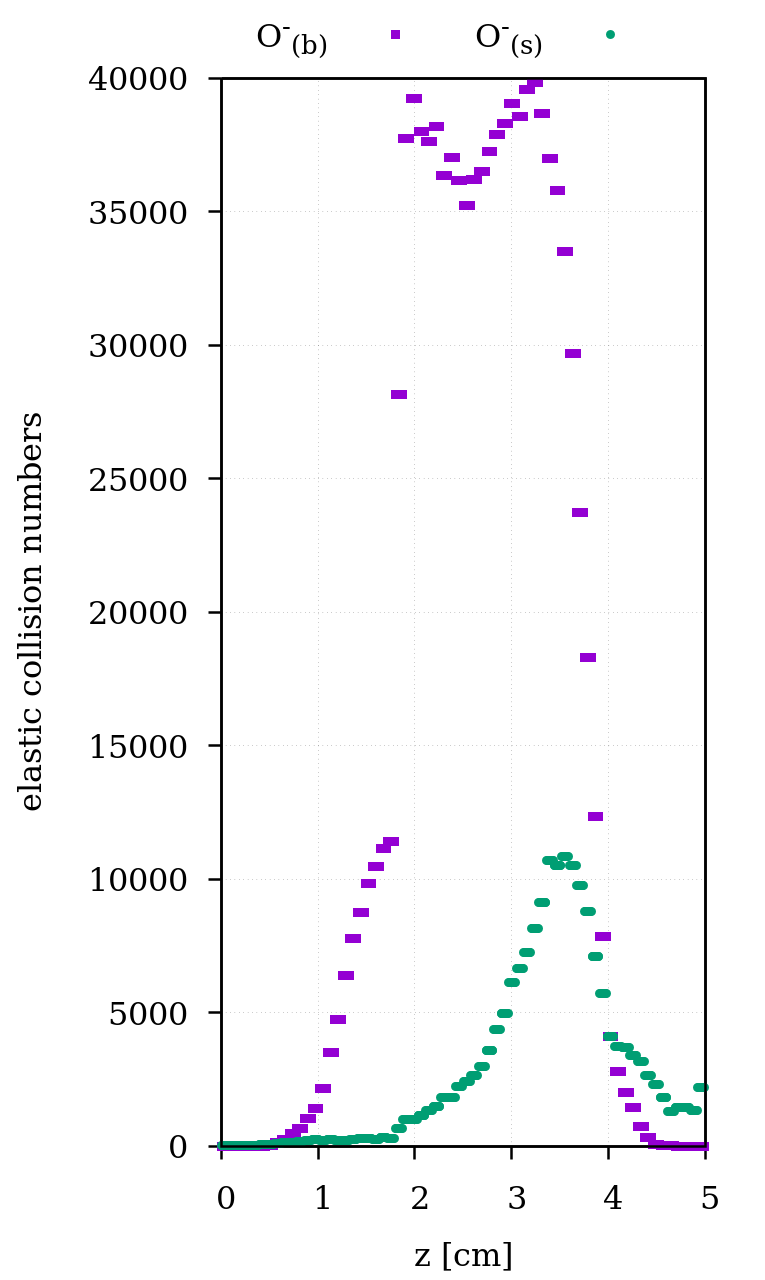
\includegraphics[width=0.42\textwidth]{figures/results/1D/elastcoll.png}
            \caption[Elastic collisions for surface and bulk anions]{%
                Elastic collisions of surface and bulk anions.}
            \label{fig:elastcoll1d}
        \end{wrapfigure}
%        
         The total number of collisions with neutral gas molecules for negative ions from the bulk and surface is shown in~\autoref{fig:elastcoll1d}. They include elastic scattering and charge exchange processes. As expected, most collisions happen in the bulk, but also some occur in the sheath at \SI{5}{cm}. Obviously the sheath is collisional. The collisions of energetic $O^{-}$ with low energy $O_{2}$ molecules at room temperature leads to a loss of kinetic energy. This is due to either elastic scattering or charge exchange processes, where the anion becomes cold when colliding with a molecule.\\
        Because I am interested in the dynamics of the plasma the energy distribution functions of the charged species are of particular interest, especially those of the surface generated $O^{-}$ ions. The next part is therefore devoted to the discussion of the particles EDF and the corresponding behaviour.
%        
    \section{Energy Distribution Functions and Anion Dynamics}
%
			The EDFs of both ion species have large particle counts at low energy values, distributed over the plasma bulk at the centre of the discharge. The corresponding kinetic temperatures for the majority of positive and negative ions are rather low, e.g\@ between $\tenpo{3}$K to $\tenpo{4}$K. This `cold core' expands from 50 to 370$\,\lambda\ix{D,e}$ and \SIrange{-5}{+5}{\electronvolt} respectively. The high energy part in the distribution function of $O^{+}_{2}$ between 0 -- 50$\,\lambda\ix{D,e}$, and 370 -- 426$\,\lambda\ix{D,e}$ is a result of the acceleration in the sheath by the potential drop of  $\approx\unit[200]{V}\,$. The low energy part of the distribution establishes through energy loss collisions and bulk ionisation processes with slow exit velocities.\\
        There are subtle structures in the positive ion EDF between electrodes and bulk below the higher energy distribution tail. One can count 7 to 8 of such characteristic peaks on both sides. This is likely the number of rf cycles an ion stays in the plasma sheath. Assuming the ion energy is approximately \SI{50}{\electronvolt} upon entering the sheath, an its thickness roughly \SI{0.75}{\centi\meter}, the transit time of the incident particle is $\approx\,$\SI{8.3} times the duration of a full radio frequency cycle. It is de-/accelerated inside the sheath, oscillating with the phase of the external electric field. Therefore, ions can gain up to 8 times the energy from the electric field in one RF cycle while passing through the sheath and flying towards the electrode. They are eventually reflected and likewise accelerated again in the opposite direction.\\
        The dynamics of the negatively charged electrons in the sheaths is very well highlighted in~\autoref{fig:edf_ex}. One can see the acceleration between 0--50$\,\lambda\ix{D,e}$, which yields energies of up to \SI{100}{\electronvolt}. The higher energy portion of the electrons from the anode traverses the bulk and is decelerated in the opposing sheath and vice versa. Also, the electron EDF has a low energy peak in the bulk between \SIrange{-50}{50}{\electronvolt}, whose numbers quickly decay to higher values due to energy loss collisions.\\
        In~\autoref{fig:edf_snix} the energy distribution of negative ions produced in the plasma bulk is shown. The form of electron and negative bulk ion EDF is similar in a sense that both show a low energy peak across the bulk length between 50 and 370$\,\lambda\ix{D,e}$. In contrast, fast electrons from the anode reach the cathode with a kinetic energy $E\ix{kin}>0$, as seen in~\autoref{fig:edf_ex}, whereas the negative ion distribution does not have this feature. Their distribution functions shows the intrinsic de-/acceleration in the sheaths of this symmetric discharge. Anions from the bulk never gain a kinetic energy large enough to pass the potential barrier at the electrodes. They are reflected at the boundary/in the sheath and eventually make it across the bulk to be reflected again.\\
        The distribution function of anions produced at the surface shows the acceleration by the potential drop in the plasma sheath, which yields kinetic energies up to \SI{120}{\electronvolt}. The corresponding peak can be found between 370 and 426$\,\lambda\ix{D,e}$ in~\autoref{fig:edf_snix}. There is also a peak at \SI{-50}/\SI{50}{\electronvolt} between 50 and 370$\,\lambda\ix{D,e}$. This is the result of fast particles being decelerated in the plasma bulk. They are reflected at the sheath edges because of their decreased kinetic energy, and therefore do not make it to the anode. Collisionless surface ions are reflected in the opposing, which is why there are similar structures to the ones discussed earlier between 0 and 50$\,\lambda\ix{D,e}$.\\
%%%%%%%%%%%%%%%%%%%%%%%
%%%%%%%% LEFT EVEN PAGE
%%%%%%%% ION AND NION
		\pagebreak
        \begin{figure}[!h]
            \centering
            \includegraphics[width=0.8\textwidth]%
				{figures/results/1D/ix_edf.png}
            \caption[Ion EDF in 1D]{%
                Logartihmic spatial-energetically %
				resolved EDF of postive ions from a discharge at %
				\SI{5}{\pascal} and \SI{400}{\volt}.}
			\label{fig:edf_ix}
        \end{figure}
				\vfill
        \begin{figure}[!h]
            \centering
        	\includegraphics[width=0.8\textwidth]%
				{figures/results/1D/nix_edf2.png}
            \caption[Negative ion EDF in 1D]{%
                Logarithmic spatial-energetically resolved EDF of negative %
                ions from a discharge at \SI{2}{\pascal} %
                and \SI{400}{\volt}.}
            \label{fig:edf_nix}
        \end{figure}
		\pagebreak
%%%%%%%%%%%%%%%%%%%%%%%
%%%%%%%% RIGHT ODD PAGE
%%%%%%%% EL AND SNION
        \begin{figure}[!h]
            \centering
            \includegraphics[width=0.8\textwidth]%
				{figures/results/1D/ex_edf.png}
            \caption[Electron EDF in 1D]{%
            	Logarithmic spatial-energetically resolved EDF of electrons %
            	from a discharge at \SI{2}{\pascal} and \SI{400}{\volt}.}
			\label{fig:edf_ex}
        \end{figure}
				\vfill
				\begin{figure}[!h]
            \centering
            \includegraphics[width=0.8\textwidth]%
					{figures/results/1D/snix_edf.png}
            \caption[Surface produced anion EDF in 1D]{%
                Logarithmic spatial-energetically resolved EDF %
                negative ions produced on the surface from %
		    	a discharge at \SI{2}{\pascal} and \SI{400}{\volt}.}
            \label{fig:edf_snix}
        \end{figure}
				\pagebreak
%                
        The surface anion EDF slightly increases towards the cathode. This is due to the asymmetric secondary ion emission, because we only considered the production of negative ions at the cathode. Additionally, there are also peaks similar to the one found for positive ions in the lower energy part of the EDF in front of the cathode. A closer look at this can be found in~\autoref{fig:snix_prs}.\\
        The~\autoref{fig:snixsurf} shows the high energy peak of the previously discussed surface anion distribution function. This structure decays with the mean free path of the negative ions. For example, the $O^{-}$ loses energy or it is lost by detachment at $O_{2}$ and recombination with $O^{+}_{2}$. This also creates the density peak in front of the cathode in~\autoref{fig:denscompare1d}. Negative ions from surfaces may become cold through energy loss collisions, which is why they eventually remain in the bulk.\\
        The subtle structure in the cathode sheath region of the surface anion EDF builds up due to the low transit time of a slow particle through the space charge area. Therefore the phase-resolved distribution function of the negative surface ions is shown in~\autoref{fig:snix_prs}. The modulation of the electrodes and sheaths potential causes de-/acceleration of the slow particles entering at approximately \SI{50}{ev}. They need \SI{4.32e-7}{\second} to travel through a sheath of thickness \SI{0.75}{\centi\meter} the given kinetic energy. It stays for roughly 5--6 rf cycles inside the sheath. This produces the same additional peak structures as for positive ions. In the phase-resolved EDF we can see anion density peaks moving according to the phase of the rf signal. Between five and six peaks are visible at a given moment in the excitation, which supports the findings from before. The ions enter the sheath easier when the voltage is positive during $\varphi\le\pi$. Afterwards they are accelerated away from the sheath at $\pi<\varphi\le2\pi$. The anions/ions oscillate back and forth. Their kinetic energy is transferred into potential energy in the sheath and vice versa.\\
        The particle numbers in the EDF of surface ions are at least one order of magnitude smaller than those of the bulk ions. This is due to the low surface production of an efficiency $\eta=\,$0.03~\cite{Meichsner13} at the cathode and low pressures of \SI{2}{\pascal}, which favours the production of anions in the plasma volume.\\
        Figure (\ref{fig:compare_ied}) confirms, in comparison with the experimental results from~\autoref{fig:expresults}, that negative ions produced at the surface may lead to the measured high-energy peak. The energy distribution function of the simulation has additional low energy peaks at $<\unit[100]{eV}$, too. They are created due to the energy loss by collisions and the intrinsic symmetry of the sheaths. This peak structure was also found and discussed for~\autoref{fig:snixsurf}.\\
        In the experiment all high-energy anions are detected by a mass-spectrometer and thereby removed from the discharge. In this simulation however, the collection of the energy distribution function does not perturb the results in any way.
%%%%%%%%%%%%%%%%%%%%%%%
%%%%%%%% LEFT EVEN PAGE
%%%%%%%% SNION CLOSE UP SURF
				\pagebreak
        \begin{figure}[!h]
            \centering
            \includegraphics[width=0.8\textwidth]%
				{figures/results/1D/snix_close_edf.png}
            \caption[Surface anion EDF close up]{%
				Same EDF as shown in~\autoref{fig:edf_snix}. %
                Close up the structures in the cathode sec:sheathphysics.}
            \label{fig:snixclose}
        \end{figure}
		\vfill
		\begin{figure}[!h]
        	\centering
        	\includegraphics[width=0.9\textwidth]%
					{figures/results/1D/snix_surface_edf.png}
            \caption[Negative ion EDF surface plot]{%
    			EDF as in~\autoref{fig:edf_snix} as a surface plot. %
    			One can see the energy peak at around\SI{-100}{\electronvolt} %
    			decaying over the length of the bulk.}
            \label{fig:snixsurf}
        \end{figure}
				\pagebreak
%%%%%%%%%%%%%%%%%%%%%%%
%%%%%%%% RIGHT ODD PAGE
%%%%%%%% PHASE RESOLVED
        \begin{figure}[!h]
            \centering
            \includegraphics[width=1.0\textwidth]%
				{figures/results/1D/snix_allpi_edf2.png}
            \caption[Phase resolved structures in the EDF of surface ions]{%
                Phase resolved surface anion energy distribution %
                functions in front of the cathode.}
            \label{fig:snix_prs}
        \end{figure}
        
        We have now thoroughly investigated the formation and dynamics of surface produced secondary anions in a 1d3v PIC simulation. It was found that surface ions have a significant impact on the energy distribution function of $O^{-}$. However, it was not seen that fast anions created at the surface of the cathode impinge onto the anode. This is due to the intrinsic acceleration in the potential of the sheath, and therefore deceleration in the opposing space charge. One can already tell this from the averaged potential in~\autoref{fig:pot1d}. A key element to the solution of this problem id the asymmetry of the driven discharge with a self bias voltage. This leads to a stronger acceleration at the cathode than retardation at the anode, and hence to the impact onto the electrode.\\
        The self consistent adjustment of plasma electron and ion current between volume and sheath makes it impossible to implement asymmetry in an one-dimensional simulations. The physics of bulk and sheath are governing the establishment of space charges, as well as the corresponding potential drops towards walls.
%
        \begin{figure}[!h]
            \centering
            \includegraphics[width=0.8\textwidth]%
				{figures/SFB/power_energy_cuts.png}
            \caption[EDF results from 1D at the anode]{%
                Energy distribution of negative ions $O^-$. Simulation result taken %
                at the anode sheath edge at different rf powers at $\unit[5]{Pa}$.}
            \label{fig:compare_ied}
        \end{figure}
%        
        Like it was discussed by Bronold and Matyash et al. in~\cite{Bronold07b}, the key argument for a one-dimensional simulation is the large electrode diameter in comparison to the electrode gap. Here it is said that the plasma properties are not affected, or at least the influence is considered negligible, by the boundaries of the electrodes. Along the axial centre of the discharge the plasma `does not see' the edge of the electrodes and therefore no asymmetry effects should take place~\cite{Matthias15}.\\
        From the results found by~\cite{Scheuer15} we know that fast ions can impinge onto the anode. Hence one needs a better model to describe the relevant physics of the experiment. A step towards this solution is the introduction of a two-dimension PIC simulation in which asymmetry effects such as self bias are implemented. The next chapter is devoted to that topic.

	%
\chapter{Simulation of capacitively coupled rf discharges}\label{sec:chapter_twodccrf}
%
	\section{Experimental setup}\label{sec:twod_setup}
%
		After introducing the basics physics in~\autoref{sec:surfaceeffects} and validating the code successfully in~\autoref{sec:chapter_onedcomparison}, the effects of highly energetic negative oxygen ions can now be further investigated with the code.
%
		\subsection{Reference Discharge}\label{sec:reference_dis}
%
			\begin{figure}[b!]
				\centering
				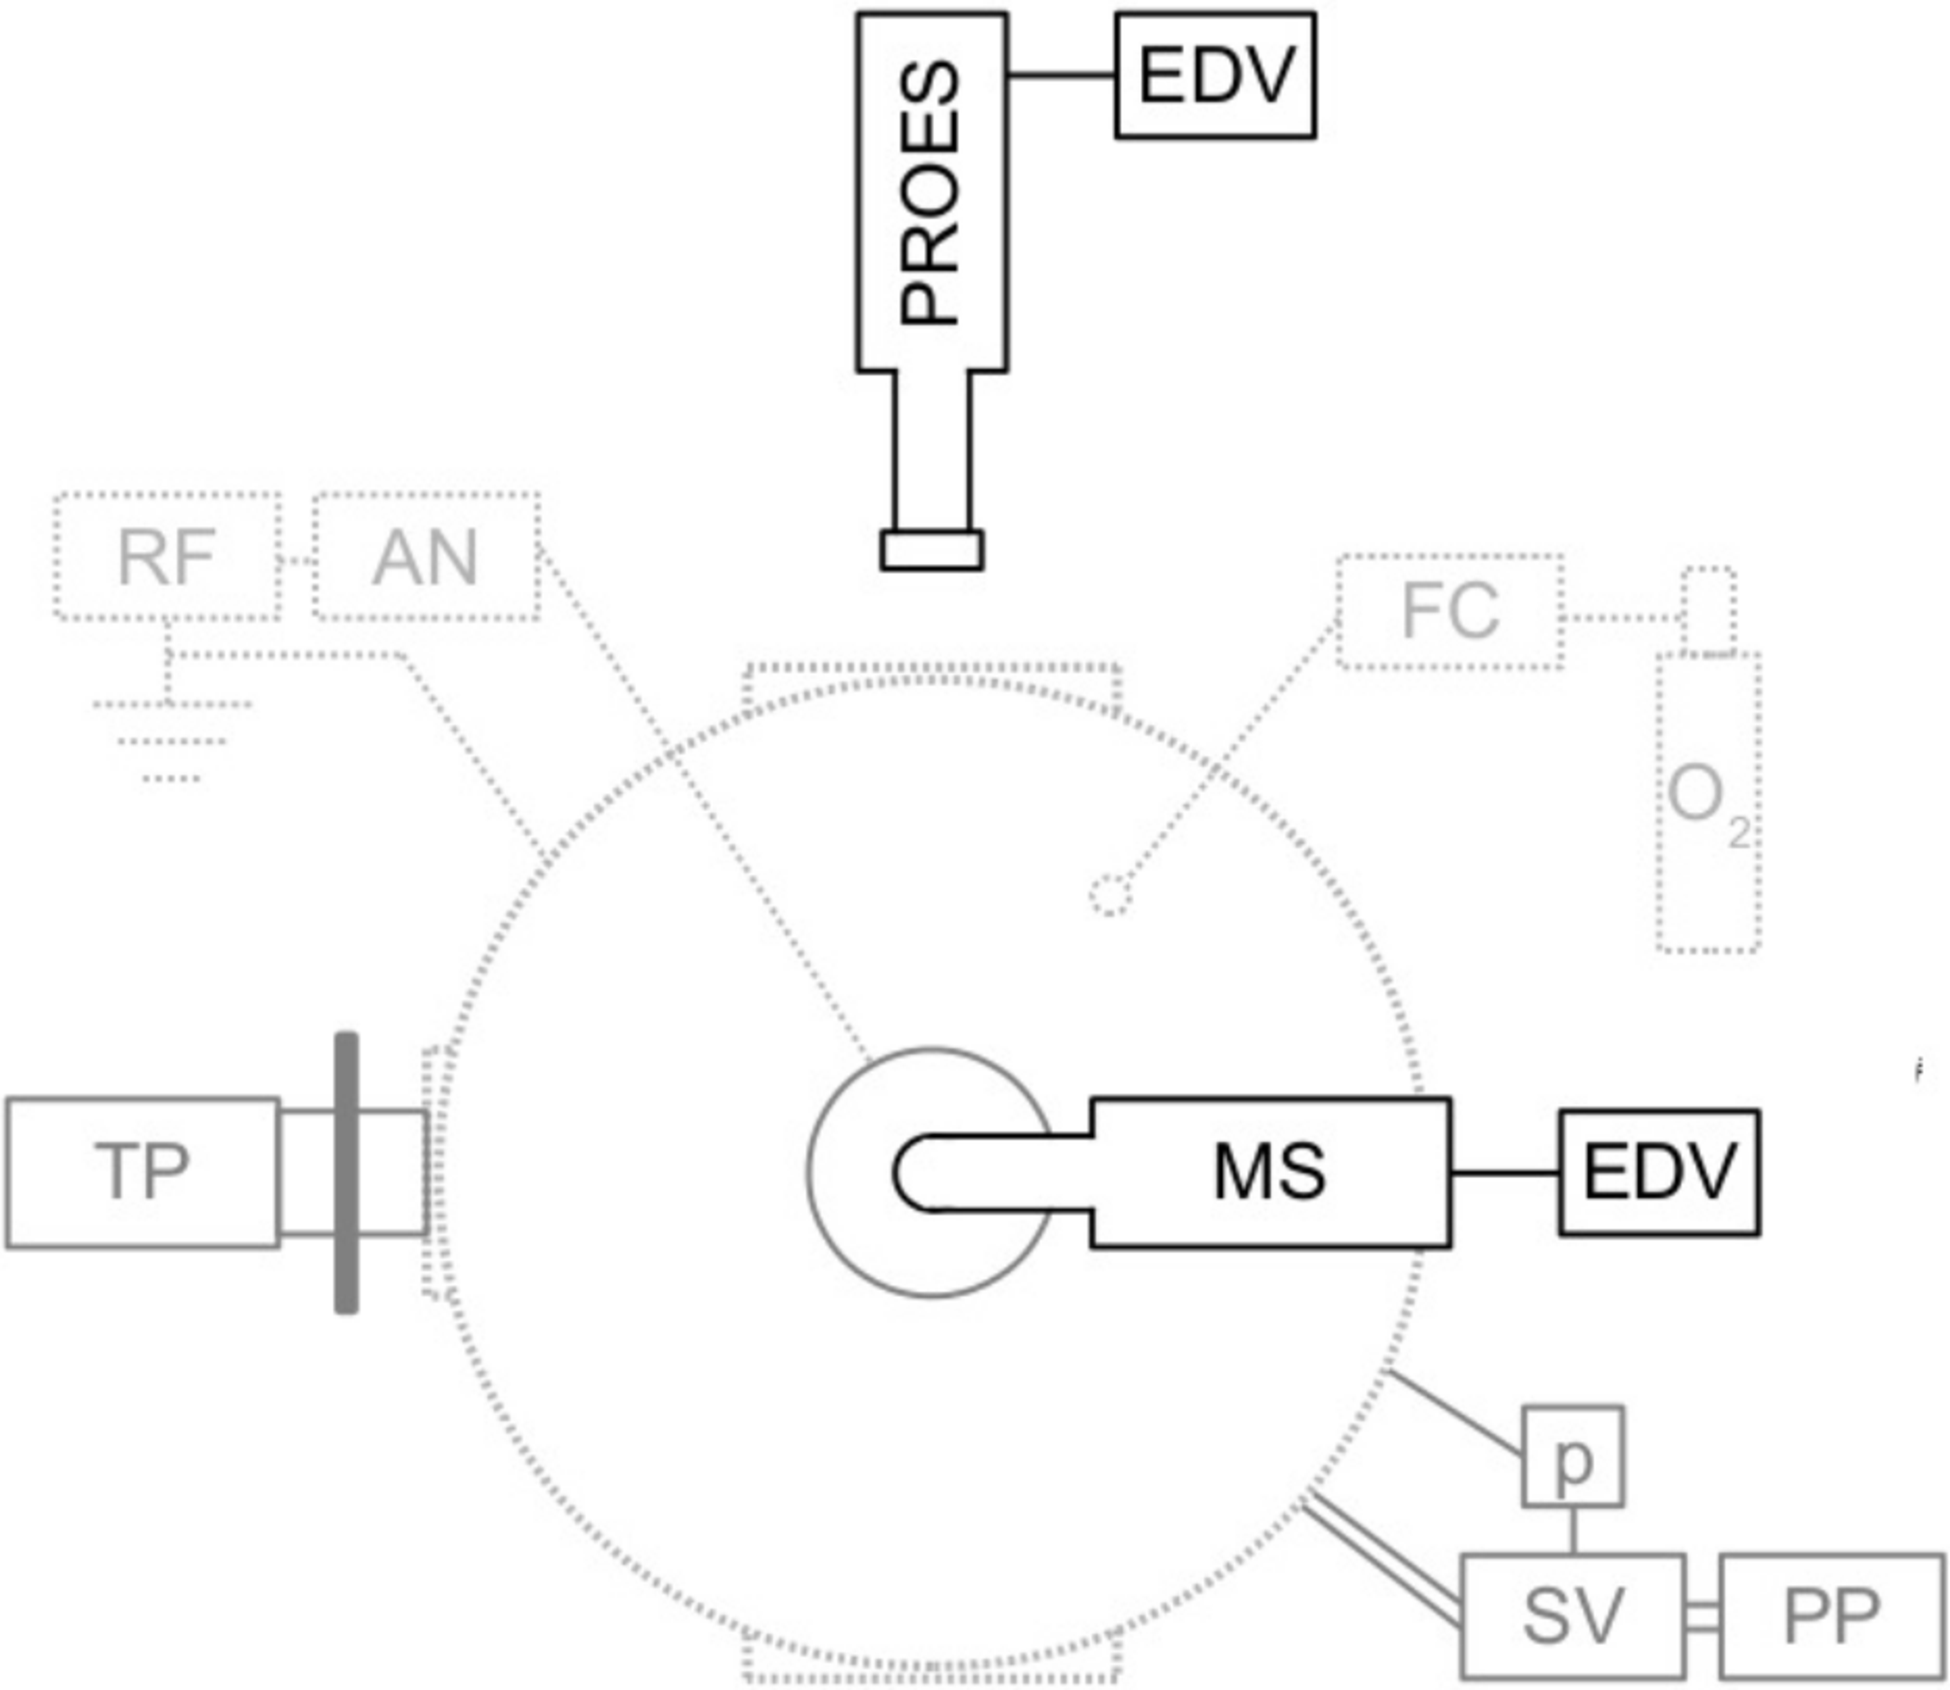
\includegraphics[width=0.5\textwidth]{figures/chamber_exp.pdf}
				\caption{%
					Top-down view schematic of the experiment~\cite{Scheuer15},~\cite{Kullig12}. Shown is the setup %
					without microwave interferometer, like it was used by Küllig et al.}\label{fig:discharge_chamber}
			\end{figure}
%
			Here, the referenced experiment was used by Küllig et al.~\cite{Kullig12} and Scheuer~\cite{Scheuer15}, and consists of a cylindrical setup, filled with oxygen at low pressures and gas flow rates (see~\autoref{fig:discharge_chamber}). The stainless steel vacuum chamber had a diameter and height of $\unit[40]{cm}$ respectively and was filled with the process gas oxygen (O$\ix{2}$) at $\unit[5]{sccm}$ (\fett{FC}). The discharge configuration consisted of an electrode in the center with $\unit[10]{cm}$ of diameter and a rf generator, constantly operating at a frequency of $\unit[13,56]{MHz}$ and power outputs between $5$ and $\unit[150]{W}$ (\fett{RF} and \fett{AN}), leading to applied voltages in the range of $100$--$\unit[1500]{V}$. Shielding and discharge enclosure/chamber walls were grounded, therefore yielding a large area ratio between driven and grounded electrode and establishing a heavily asymmetric plasma. In addition, the powered electrode was coupled capacitively with the external generator, emphasizing the effect of the, in~\autoref{sec:selfbias} introduced self bias voltage. The value of $U\ix{sb}$ ranged, depending on power output and discharge pressure, from $-100$ up to $\unit[500]{V}$. In~\cite{Kullig12} the experiment was pulsed with short discharges at a frequency of $\unit[10]{Hz}$.	Line integrated measurements resulted in an average electron density of around $\tenpo{11}$--$\unit[\tenpo{12}]{cm^{-3}}$. Showing a schematic top-down view of the experiment is~\autoref{fig:discharge_chamber}. Here, the large ratio between driven and grounded parts is very well visualized. Hence, in later simulations it will be of sufficient accuracy to restrain the virtualized volume to a smaller setup.\\
			The figure below includes further diagnostics like a mass spectrometer (\fett{MS}) and phase resolved optical emission spectroscopy (\fett{PROES}). The latter measured the mentioned densities via line integration across the plasma volume. The MS is a key instrument for the investigation pursued in this thesis, as it also measures species counts with respect to their contribution to their corresponding energy distribution function. For example, the ions created via secondary processes in the discharge sheath are accelerated towards the bulk and thus get into the MS with their characteristic speeds and mass. A significant increase of electron density was found for rf powers larger than $\unit[50]{W}$ or $\unit[-220]{V}$ self bias voltage~\cite{Kullig12}. This led to a correlating negative oxygen ion density reduction and decrease of the electronegativity ratio $\overline{n}_{i,-}/\overline{n}\ix{e}$ from $4$ to $0,03$. During a different operation mode --- called $\alpha$-mode, contrary to the afore-mentioned $\gamma$-mode --- at less than $\unit[50]{V}$ output power, electronegativity rises again, as well as the electron temperature $T\ix{e}$, yielding higher rate coefficients for, e.g.\@ dissociative electron attachment and the alike. See~\autoref{sec:anionproduction} for a more detailed approach.
%
		\subsection{Simulated Discharge}\label{sec:simulatedd_dis}
%
			All of the above conditions are sufficient for a practical approach at a labratory ccrf discharge with great repeatability. Though being highly optimized and developed over the course of many years, the twodimensional particle-in-cell code outlined above does not provide the tools and performance to feasibly simulate such large areas and particle numbers. Hence, one will reside to reducing the numerical expense by virtualizing smaller discharge areas and average densities, while trying to satisfy the same physical processes exhibited in~\cite{Kullig12}.\\
			The afore-mentioned 2d3v PIC code is used to simulated the referenced experiment. The spatial dimensions will be the radial component $r$ and axial coordinate $z$. The geometry and simulation is optimized for cylindrically symmetric gas discharges.\\
			To represent the strong asymmetry between driven and grounded wall areas, the sizes of anode, cathode and grounded chamber parts have been chosing accordingly. The experimental values for the self bias voltage $U\ix{sb}$ were used to create a dc offset on-top of the rf voltage $U\ix{rf}$ at the cathode. The domain composition with cells of width $\lambda\ix{D,e}/2$ (see~\autoref{sec:picbasics}) makes it even more difficult to appropriately model the system. Hence a smaller discharge volume of a $\unit[4,5]{cm}$ radius and an electrode gap of $\unit[2,5]{cm}$ will be simulated. This usually leads to cell counts up to $2\cdot\tenpo{5}$, which is small in comparison to the `real' experiment, which would have to be covered by over $\tenpo{6}$ cells. Furthermore, the numerical expense grows with $N\log(N)$, and $N$ being the particle number inside the cells (see~\autoref{sec:picsimulationmcc}).\\
			One has chosen pressures between $\unit[2]{Pa}$ and $\unit[10]{Pa}$, with the possibility of changing it later during the discharges simulation --- e.g\@ to change the bulk volume and densities. The secondary ion emission efficiency was set to $\eta=0,03$ in all cases, yielding a stable plasma sheath and hence SIE current into the bulk. In addition, a constant self bias of $\unit[-200]{V}$ was appplied at the cathode. The radio frequency was set to $\unit[13,56]{MHz}$.\\
			The governing electron density and temperature were set to $\unit[5\cdot\tenpo{9}]{cm^{-3}}$ and $\unit[5]{eV}$ respectively, which, as an initial value and property for scale, is sufficient for the necessary rate coefficients mentioned above. This led to the following important scales of simulation: 
%
			\begin{align}
				\lambda\ix{D}&=\unit[0,0235]{cm}\,,%
				\hspace*{2.0cm}%
				\omega\ix{p,e}=\unit[3,99\cdot\tenpo{9}]{Hz}%
				\label{equ:debyeandomega}\\[0.0cm]
				\Rightarrow \Delta x&=\frac{1}{2}\,\lambda\ix{D}=\unit[0,01174]{cm}\,,%
				\quad\quad%
				\Delta t=0,2\cdot\omega\ix{p,e}=\unit[5,015\cdot\tenpo{-11}]{s}%
				\label{equ:simulationscales}
			\end{align}
%			
			Thus a single rf cycle at the given frequency takes $1470$ steps, and the domain measures $384$ and $213$ in radial and axial dimension respectively. An ion temperature is adjusted via the fraction $T\ix{i}/T\ix{e}=0,008$, hence the corresponding velocities for the previously defined electron temperature $T\ix{e}=\unit[5]{eV}=\unit[5,8\cdot\tenpo{4}]{K}$ are found to be
%
			\begin{align}
				v\ix{th,e}=&\,\unit[9,37\cdot\tenpo{5}]{\frac{m}{s}}\,,%
				\quad\quad%
				c\ix{s,e}=\,\unit[3,87\cdot\tenpo{3}]{\frac{m}{s}}%
				\label{equ:electronvelocities}\\[0.0cm]%
%				IONS 
				v\ix{th,i}=&\,\unit[558,38]{\frac{m}{s}}\,,%
				\hspace*{1.2cm}%
				c\ix{s,i}=\,\unit[371,44]{\frac{m}{s}}%
				\label{equ:ionvelocities}
			\end{align}
%
			\begin{wrapfigure}{r}{0.3\textwidth}
				\centering
				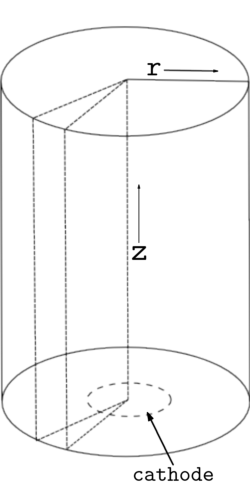
\includegraphics[width=0.275\textwidth]{figures/radial_cylinder.pdf}\\
				\vspace*{0.3cm}\hspace*{0.1cm}
				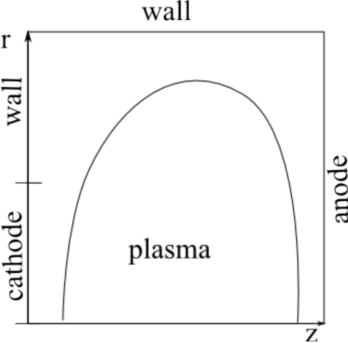
\includegraphics[width=0.275\textwidth]{figures/domain_slice.pdf}
				\caption{%
					Simplified cylinder schematic for the simulated experiment. The slice depicte in the top %
					is shown below. There, boundaries and bulk position are outlined.}\label{fig:radialcylinder}
			\end{wrapfigure}
%
			Here, a single millisecond of operation takes days, if not weeks to simulate with a given timestep, like in~\autoref{equ:simulationscales}. Due to this and the fact, that the unit cell volume increases with the layer index of the radial coordinate --- one has to keep in mind that the cylindrical geometry is key to the simulation because important simplifications and assumptions inside the code itself are made uppon that premise ---, each particle carries an additional statistical weight. For example, a virtual neutral gas molecule of O$\ix{2}$ may represents up to $\tenpo{8}$ `real' particles in a laboratory plasma. This saves a vast amount of computational time by immensely reducing the particle counts necessary to sufficiently model the investigated physical processes. In this case, a single neutral gas particle is statistically amplified by a factor of $\approx 9,3\cdot\tenpo{7}$ to account for the gas density at $\unit[5]{Pa}$ and $\approx\unit[300]{K}$. This number is crucial to all collisional processes, where the molecular species O$\ix{2}$ is involved. Charged particle species share a common number amplification of $8489$. On top of both super particle factors, a scaling $\sim 1/r$ is applied to consider the variable cell volume.\\
			Another assumption in the simulation is a constant neutral gas background. In the experiment, a working gas reservoir and flow rate meter control the pressure and exchange of O$\ix{2}$ inside the chamber. The cold neutral species has a very slow drift velocities, and therefore a large time scale of the transport process in the range of a couple $\unit{ms}$. Also the mean-free-paths are very large and collisions do not change the neutral gas distribution. Hence, the O$\ix{2}$ molecules are initiated at time $t=0$ of the simulation --- this is done with respect to pressure, super particle factor and volume weighting  ---, and are afterwards not altered in number or location. Though collision routines are still exercised, the corresponding push of the neutral species is skipped.
%
	\section{Simulated ccrf Oxygen Discharge}\label{sec:twod_secondaryions}
%
		In the collection of~\autoref{fig:2d-collection} twodimensional densities and potential are shown. Again, parameters were chosen as $U\ix{rf}=\unit[400]{V}$, $p=\unit[5]{Pa}$ and the initial species attributes to be $T\ix{e}=\unit[5]{eV}$, $n\ix{e,0}=\unit[5\cdot\tenpo{9}]{cm^{-3}}$ and $T\ix{i}/T\ix{e}=0,008$ respectively. 
%  
	\section{Anion Energy Distributions in Oxygen}\label{sec:twod_negionsdist}
%

% END
	%
\chapter*{Conclusions}\label{sec:chapter_conclusion}
\addchaptertocentry{Conclusion}
%
%
%   !!!WAS FEHLT: AUFGREIFEN DER HAUPTFRAGESTELLUNGEN AUS DER EINLEITUNG UND KLARE BEANTWORTUNG DER FORSCHUNGSFRAGEN, 
%   DIE DORT FORMULIERT WURDEN.
%   ICH WÜRDE DIE BEIDEN FRAGEN EXPLIZIT NENNEN UND DANN KLAR UND PRÄZISE BEANTWORTEN!!!
%
%
    In my thesis I applied a 1D and 2D Particle-in-Cell algorithm including Monte-Carlo-Collisions to simulate a cylindrical low-temperature ccrf discharge at low pressures of oxygen. The goal was to investigate the experimental findings from~\cite{Scheuer15}, where highly energetic anions were measured by a mass-spectrometer at the anode of a ccrf oxygen discharge. An explanation is proposed by Stoffels and Kawano et al.~\cite{Stoffels01,Kawano83}, suggesting that negative ions are produced by atomic or molecular neutral particles at the electrode surfaces.\\
    A 1D PIC model was used to understand the basic plasma physics and dynamics of negative ions including this surface process at the cathode. An estimate for the efficiency of secondary ion emission was made from experimental results~\Cite{Meichsner13}. I was able to reproduce qualitatively the energy distribution function of negative ions, which has a high energy peak due to the acceleration of secondary ions in the plasma sheath. A plateau and an additional low-energy peak in the EDF build up due to energy loss collisions in the bulk and sheath.\\
    However, I was not able to find anions from the cathode to impinge on the anode. This was due to the intrinsic symmetry of a 1D simulation. Hence a 2D simulation model was needed, in which asymmetry effects can occur and a self bias voltage can be applied.\\
    The 2D code was then validated by comparison with the 1D model. It could be shown that both simulations are in good agreement.\\
   In the 2D simulation asymmetrical driven discharges are studied, where cathode and anode configurations are varied and the self bias is introduced. Here, I found that the plasma adjusts self consistently to the different boundary configurations by re-shaping the sheaths and balancing particle currents for the global continuity condition. In case of a highly asymmetric discharge, where the plasma is in contact with a larger area of grounded walls, the sheaths are deformed to match this requirement. They are much larger in front of grounded walls than at a driven electrode. Also the decrease of bulk density and potential is more shallow there. This leads to the reduction of particle densities and velocities inside to balance the flux.\\
   Accordingly, the EDFs of the plasma species adopt and show the characteristic found in the experiment. Negative ions produced at the cathode can impinge on the opposing anode, because the self bias voltage offset creates an asymmetric acceleration, which lets the anions overcome the potential barrier in front of the grounded wall. The lower energy peak in the EDF of negative ions, which exists in 1D and is seen the experiment, disappears because absorption on the anode is considered.\\
    In summary, with respect to the scientific questions formulated in the beginning of this thesis, I could show that the physics and the dynamics of a ccrf low-pressure oxygen discharg is a complex balance of fast electrons and heavy positive and negative ions. The 1D PIC-MCC gave already a detailed understanding of the physics of this system. However, it lacks the possibility of asymmetries, which are necessary for realistic simulations of experiments. The 2D PIC-MCC code allows this kind of detailed comparison.\\
    This 2D PIC-MCC code gives detailed insight into the second research question, namely to understand the EDF of surface produced secondary particles, like negative oxygen ions. They gain a high energy by a strong acceleration in the sheath. The self bias voltage introduces an asymmetric acceleration of charged particles at the powered electrode. This results in a high particle count of negative ions at large kinetic energies as it is also observed experimentally at the grounded anode. Energy loss and charge exchange collisions lead to the broadening of this peak already in the plasma sheath, which creates a plateau over large ranges of energy. This can be seen in~\autoref{fig:twodedf_ni}, which is very close to the experimental measurements.
Therefore, the two major questions formulated at the beginning of the thesis could be addressed successfully.
%
    \par%
    In the future, the 2D PIC simulation can be used to study further aspects of asymmetric electronegative discharges, e.g. introducing complex sputter models including chemical reactions. This will also allow to apply it to industrial applications like etching for a more detailed microscopic description. Also, a self consistent approach for the self bias voltage may be implemented. One could measure the flux and accumulated charge locally and thereby calculate an individual dc voltage offset. The displacement current between sheath and bulk is used to approximate the self bias voltage in a balance of inward and outward charge current. Experiments might yield the relevant sheath capacities for the calculation of the self bias. Surface processes are still not very well studied theoretically and experimentally. If here more knowledge exist,  emission probabilities for surface processes from theory or experiment can be implemented.
	%\chapter{Epilogue}

	\section{Local electrostratic field solver}

  \section{Diagnostics of current and charge}
  
  \section{Field calculation}

  \section{Comparison with Poisson-based solvers}

% ************************************************************************** %
%	
% ************************************************************************** %
% APPENDICES
	\appendix % Cue to tell LaTeX that following "chapters" are Appendices
	% Include the appendices of the thesis as separate files
	% Uncomment the lines as you write the Appendices
	\chapter{Appendix}
%
% ************************************************************************** %
% PHYSICAL PROPERTIES
  \section{Physical Properties}
  \begin{longtable}{m{0.32\textwidth}m{0.32\textwidth}m{0.32\textwidth}}
    \toprule
    \bfseries quantity & \bfseries equation & \bfseries relevance \\%
    \toprule\midrule\endhead%
      Debye length &%
        $\begin{aligned}
          \lambda\ix{D,j}^2&=\frac{\varepsilon\ix{0}k\ix{B}T\ix{j}}{n\ix{j}e^2} \\
          \lambda\ix{D}^2&={\left(\lambda\ix{D,e}^{-2}+\lambda\ix{D,i}^{-2}\right)}^{-1}
        \end{aligned}$ &%
          distance around a charge, at which quasi-neutrality is satisfied, %
          $\lambda\ix{D}$ is the combined screening length from individual species \\ \midrule%
      plasma parameter &%
        $\begin{aligned}
          N\ix{D} = n\frac{4}{3}\pi\lambda\ix{D}^{3}
        \end{aligned}$ &%
        number of particles inside Debye sphere, if $N\ix{D} \gg 1$ an ionized gas %
        is considered a plasma (degree of ionization) \\ \midrule%
      plasma frequency &%
        $\begin{aligned}
          \omega\ix{p,j}^2=\frac{n\ix{j}e^2}{\varepsilon\ix{0}m\ix{j}}=%
          \frac{v\ix{th,j}}{\lambda\ix{D,j}}=\frac{1}{\tau\ix{j}}
        \end{aligned}$ &%
          upper limit for interaction with fields/forces or external excitations %
          inverse screening time \\ \midrule%
      thermal velocity &%
        $\begin{aligned}
          v\ix{th,j}^2=\frac{k\ix{B}T\ix{j}}{m\ix{j}}
        \end{aligned}$ &%
          mean velocity from kinetic theory of gases \\ \midrule%
      coulomb logarithm &%
        $\begin{aligned}
          &\ln\left(\Lambda\right) \\ \\
          &\Lambda=\frac{b\max}{b\min}= \\ \\
          &\lambda\ix{D}\cdot%
          \frac{4\pi\varepsilon\ix{0}\mu v\ix{th}^{2}}{e^{2}} 
        \end{aligned}$ &%
          dimensionless scale for transport processes inside discharge \newline
          fraction of probability for a cumulative $90^{\circ}$ scattering by many small %
          pertubation collisions and a single right angle scattering \\ \midrule%
      collision frequency &%
        $\begin{aligned}
          \nu\ix{j}=\frac{e^{4}n\ix{j}\ln\left(\Lambda\right)}%
          {8\sqrt{2m\ix{j}}\pi\varepsilon\ix{0}{\left(k\ix{B}T\ix{j}\right)}^{3/2}}
        \end{aligned}$ &%
          two body coulomb collision frequency inside species j \\ \midrule%
      particle distance \& \newline mean free path &%
        $\begin{aligned}
          &\overline{b}=\frac{\hbar}{m\ix{j}v\ix{th,j}} \\ \\
          &s\ix{mfp,j}=\frac{v\ix{th,j}}{\nu\ix{j,k}}
        \end{aligned}$ &%
          mean inter particle distance for species j \newline% 
          free flight between subsequent collisions of species j and k %
          with collision frequency $\nu\ix{j,k}$ \\ \midrule%
      speed of sound &%
        $\begin{aligned}
          c\ix{S}^{2}&=\frac{\gamma Zk\ix{B}T\ix{e}}{m\ix{i}} \\
          \gamma&=1+2/f=5/3
        \end{aligned}$ &%
        speed of longitudinal ion waves at electron pressure \newline%
        adiabatic coefficient with f, the kinetic degree of freedom\\ \midrule%
      Debye-Hückel potential &%
        $\begin{aligned}
          \Phi=\frac{Q}{4\pi\varepsilon|\vec{r}|}%
          \euler^{-\frac{|\vec{r}|}{\lambda\ix{D}}}
        \end{aligned}$ &%
        electrostatic potential of charge particle $Q$ at distance $|\vec{r}|$, \newline%
        equal to coulomb interaction with additional%
        shielding by charged particles \\ \midrule%
      drift velocity &
        $\begin{aligned}
          v\ix{d,j}=u\ix{j}=\frac{j\ix{j}}{n\ix{j}q}=\frac{m\sigma E}{\rho ef}
        \end{aligned}$ &%
        average velocity of a particle in a conductor with an electric field applied E, \newline%
        where $N$ is the number of free electrons per atom \\%
      electric mobility &
        $\begin{aligned}
          \mu\ix{j}=\frac{v\ix{d}}{E}
        \end{aligned}$ &%
        ability of charged particle of moving through an electric field \\%
    \midrule\bottomrule%
    \caption[Selection of physical properties of a low temperature ccrf discharge]{%
      Selection of physical properties of a low temperature ccrf discharge. The index $j$ denotes the %
      species, e.g.\@ electrons, ions. Used quantities can be found in the preface %
      in~\autoref{tabe:physicalconstants}.}\label{tabe:physicalquantities}
  \end{longtable}
% ************************************************************************** %
%   
		\clearpage
    \section[Energy Distributions from 2D PIC]%
            {Simulated Energy Distribution\\
            Functions from 2D PIC}\label{sec:appendix_results}
%
        \begin{center}
            \begin{figure}[!h]
                \centering
                \begin{subfigure}{0.49\textwidth}
									\includegraphics[height=0.3\textheight]%
                        {figures/results/2D/44332/e_dens.png}
                \end{subfigure}
                \begin{subfigure}{0.49\textwidth}
									\includegraphics[height=0.3\textheight]%
                        {figures/results/2D/44426/e_dens.png}
                \end{subfigure}
                %\caption[2D electron and ion density]{%
                %    Electron density from the two previously %
								%		described asymmetric 2D simulations.}
                %\label{fig:app_dens}
            %\end{figure}
						%\begin{figure}
								%\centering
                \begin{subfigure}{0.49\textwidth}
									\includegraphics[height=0.3\textheight]%
                        {figures/results/2D/44332/ni_dens.png}
                \end{subfigure}
                \begin{subfigure}{0.49\textwidth}
									\includegraphics[height=0.3\textheight]%
                        {figures/results/2D/44426/ni_dens.png}
                \end{subfigure}
								\newline
                %\caption[2D electron and ion density]{%
                %    Negative ion density from the two previously %
								%		described asymmetric 2D simulations.}
                %\label{fig:app_dens_ni}
            %\end{figure}
						%\begin{figure}[!b]
                %\centering
                \begin{subfigure}{0.49\textwidth}
									\includegraphics[height=0.22\textheight]%
                        {figures/results/2D/44332/e_distz.png}
                \end{subfigure}
                \begin{subfigure}{0.49\textwidth}
									\includegraphics[height=0.22\textheight]%
                        {figures/results/2D/44426/e_distz.png}
                \end{subfigure}
               	\caption[Electron and negative ion panel]{%
									\fett{Top}: electron density, \fett{Mid}: negative ion density, %
									\fett{Bottom}: axial compontent of electron EDF from a 2D simulation %
										of the two asymmetrical discharges discussed before-hand.}
                \label{fig:app_dens}
            \end{figure}
						\clearpage
            \begin{figure}
                \centering
                \begin{subfigure}{0.49\textwidth}
                    \includegraphics[width=1.0\textwidth]%
                        {figures/results/2D/44332/i_distz.png}
                \end{subfigure}
                \begin{subfigure}{0.49\textwidth}
                    \includegraphics[width=1.0\textwidth]%
                        {figures/results/2D/44426/i_distz.png}
                \end{subfigure}
                \caption[Axial ion EDF from 2D]{%
                    Axial compontent of ion EDF from a 2D simulation %
										of the two asymmetrical discharges discussed before-hand.}
                \label{fig:app_edf_i}
            \end{figure}
						\vfill
            \begin{figure}
                \centering
                \begin{subfigure}{0.49\textwidth}
                    \includegraphics[width=1.0\textwidth]%
                        {figures/results/2D/44332/ni_distz.png}
                \end{subfigure}
                \begin{subfigure}{0.49\textwidth}
                    \includegraphics[width=1.0\textwidth]%
                        {figures/results/2D/44426/ni_distz.png}
                \end{subfigure}
                \caption[Axial negative ion EDF from 2D]{%
                    Axial compontent of negative ion EDF from a 2D simulation %
										of the two asymmetrical discharges discussed before-hand.}
                \label{fig:app_edf_ni}
            \end{figure}
        \end{center}
%
		\clearpage
    \listoffigures % Prints the list of figures
	\listoftables % Prints the list of tables

% ************************************************************************** %
%
% ************************************************************************** %
% BIBLIOGRAPHY
	\printbibliography[heading=bibintoc]
% ************************************************************************** %
%
% ************************************************************************** %
% ACKNOWLEDGMENTS
	\pagestyle{plain}
	\begin{acknowledgements}
	% \addchaptertocentry{\acknowledgementname}
		The acknowledgments and the people to thank go here, don't forget to
	 	include your project advisor\ldots
	 \end{acknowledgements}
% ************************************************************************** %
%
% ************************************************************************** %
% INSERT MOTIVATIONAL QUOTE
%	\vspace*{0.33\textheight}
%	\rule{\textwidth}{0.1pt}
%	\noindent\enquote{%
%		Without encroaching upon grounds appertaining to the theologian and the
%		philosopher, the domain of natural sciences is surely broad enough to
%		satisfy the wildest ambition of its devotees. $\left[\dots\right]$
%		The work may be hard, and the discipline severe; but the interest never
%		fails, and great is the privilege of achievement.
%	}\bigbreak%
%	\begin{flushright}
%		--- John William Strutt, 3rd Baron Rayleigh, 1884\\
%		\small\emph{in: Address to the British Association in Montreal}
%	\end{flushright}
% \vspace*{0.15\textheight}
% \rule{\textwidth}{0.1pt}
% ************************************************************************** %
% END OF DOCUMENT
\end{document}  
% test bibliography for completion
\bibliography{master_thesis.bib}
